\documentclass[a4paper,11pt]{article}
\usepackage[left=2cm, top=2.5cm, bottom=2.5cm, right=2cm]{geometry}
\usepackage{mathpazo}
\usepackage[parfill]{parskip}
\usepackage[intlimits]{amsmath}
\usepackage{graphicx}
\usepackage{bm}

% colour text for comments etc
\usepackage{color}
\usepackage[usenames,dvipsnames,svgnames,table]{xcolor}

% micron units with \textmu
\usepackage{textcomp}

% uncurly quotes in verbatim environments (ie, for code)
\usepackage{upquote}

% adjustwidth
\usepackage{changepage}

% chemical formulae using \ce{}
\usepackage[version=3]{mhchem}

\usepackage{hyperref}
\hypersetup{colorlinks=true,citecolor=black,filecolor=black,linkcolor=black,urlcolor=blue}

\usepackage{natbib}
\bibpunct{(}{)}{;}{a}{}{,~}
\renewcommand\bibname{References}

% some maths macros - vector, derivative, partial derivative
\newcommand{\vv}[1]{\mathbf{#1}}
\newcommand{\dd}[2]{\frac{d #1}{d #2}}
\newcommand{\pd}[2]{\frac{\partial #1}{\partial #2}}

\def\slantyfrac#1#2{
\hspace{3pt}\!^{#1}\!\!\hspace{1pt}/\hspace{2pt}\!\!_{#2}\!\hspace{3pt}
}

% fourier transforms
\newcommand{\ft}[1]{\mathcal{F}\!\left\{#1\right\}}
\newcommand{\ift}[1]{\mathcal{F}^{-1}\left\{#1\right\}}
\newcommand{\iftb}[1]{\mathcal{F}^{-1}\Big\{#1\Big\}}

% argmax, argmin...
\DeclareMathOperator*{\argmax}{argmax}
\DeclareMathOperator*{\argmin}{argmin}

% table of contents control
\usepackage[nottoc]{tocbibind}
\setcounter{tocdepth}{2}

\title{BCMD modelling system 0.6b}
\author{Matthew Caldwell}

\begin{document}

\maketitle

\tableofcontents

\section{Introduction}\label{intro}

BCMD is intended to be a more portable and robust successor to the BRAINCIRC modelling environment \citep{Banaji:nuJzrisf}. Like BRAINCIRC, its primary purpose is to translate a description of a model in terms of equations and reactions into executable code that can simulate the model's behaviour for specified initial conditions and time courses of parameter changes.

Ultimately, all supported models are converted into a standard differential-algebraic equation representation, of the form:
\begin{equation}\label{eq:general}
\vv{M} \dd{\vv{y}}{t} = \vv{f}(\vv{y},\bm{\theta},t)
\end{equation}

where $\vv{y}$ is a vector of variables of interest, $\vv{M}$ is a constant, possibly-singular, mass matrix specifying relations among the differential terms, and $\vv{f}$ is some vector-valued function, possibly having additional parameters $\bm{\theta}$. (If a row of $\vv{M}$ is zero, the corresponding equation in $\vv{f}$ is algebraic rather than differential.)

The differential and algebraic equations may be specified explicitly, but it is often convenient to describe some or all of a system in terms of reacting chemical species in one or more spatial or functional compartments, as in this example from the BrainSignals model \citep[Appendix C]{Moroz:2013wx}:

\begin{equation}
p_2 \; \ce{H+_m ->[f_2] 4 Cu_{A,o} + 4 cyta_{3,r}}
\end{equation}

We attempt to make such specifications as concise and intuitive as possible, within the constraints of efficient parsing. The following code snippet declares both an explicit differential equation and the above chemical reaction in the BCMD modelling language:

\begin{verbatim}

        # the BrainSignals "v_prel" differential equation
        v_p' = 1/t_p*(P_a - v_p)
    
        # the BrainSignals "a_ox" reaction
        p2 [H, m] -> 4 [CuA_o] + 4 [cyta3_r] {f2}
        
\end{verbatim}

The modelling language is described in detail in \S\ref{models}, and a number of complete models are supplied in the \texttt{examples} directory of the BCMD distribution.

In addition to the model equation system, a model may also include arbitrary intermediate variables and parameters. Default initial values may be specified for these values, or they may be set at any step of a simulation. Unlike BRAINCIRC, BCMD does not distinguish between different types of run: as detailed in \S\ref{input}, the time course of a simulation is just driven by its input file.

\section{System requirements}\label{reqs}

BCMD runs on Linux, Mac OS X and probably other Unix-esque systems, and also on Microsoft Windows with the help of the MinGW development tools.

Models are translated to ANSI C code, so a suitable C compiler is needed to generate the model executable. Because the underlying RADAU5 DAE solver is written in Fortran, a Fortran compiler is also required to build it, and the C compiler must be capable of linking to the Fortran library. The GNU compiler toolchain (\texttt{gcc, gfortran, gmake}) is recommended, though other compilers might also work.

The included \texttt{configure} script should be able to identify the C and Fortran compilers and identify the appropriate compiler and linker options. The script is generated with \texttt{autoconfig}. If for some reason you need to recreate \texttt{configure}, the GNU \texttt{autotools} will be required; usually this should only be necessary for the package maintainers.

The model compiler is written in Python, and has been mostly tested with Python 2.7, although it may also work with Python 3.x and possibly with earlier versions. The compiler makes use of the PLY lexer/parser package \citep{PLYPythonLexYacc:n3B3Rbqj}; this is included in source code form, so no separate installation is necessary.

The compiler can optionally generate a graph of the model structure in the \href{http://www.graphviz.org}{GraphViz} DOT language. To convert this to an actual graphic image, you will need to have the GraphViz tools installed. Note that this is not necessary to be able to run models, but it can be a useful aid to analysing them.

Some additional resources are necessary in order to use the \hyperref[bgui]{BGUI graphical interface} and/or the \hyperref[batch]{batch processing utilities}. BGUI makes use of the \href{https://wiki.python.org/moin/TkInter}{Tkinter} windowing toolkit and the \href{http://matplotlib.org}{matplotlib} plotting library, while both sets of tools require the \href{http://www.numpy.org}{NumPy} numerical libraries. These packages may already be available in your Python system, but if not, the easiest way to obtain a complete installation of the whole SciPy stack is via the \href{https://www.enthought.com/products/canopy/}{Enthought Canopy} distribution---the free Canopy Express package includes all the required components.

To perform sensitivity analysis, the \href{http://jdherman.github.io/SALib/}{SALib} Python package is required; this can be installed via \texttt{pip} or manually (it is a straightforward pure Python package). For parameter optimisation, you need the \href{http://openopt.org/}{OpenOpt} framework---see the \href{http://openopt.org/install}{installation} page for information about how to install this. (The preferred option is to use \texttt{easy\_install}, but getting this to work with Enthought can be fiddly.) Ideally you should also add the \href{http://www.norg.uminho.pt/aivaz/pswarm/}{PSwarm} solver---download the PPSwarm\_v1\_5.zip code archive and build it with Python support enabled. This can be installed globally or placed directly into the BCMD distribution after you have installed the latter---put the built PSwarm python module (e.g. \texttt{pswarm\_py.so}) into the BCMD \texttt{batch/pylib} directory.

In order to support export to (and perhaps in future import from) SBML, the \href{http://sbml.org/Software/libSBML}{libSBML} library \citep{Bornstein:2008id} is required, including its Python bindings. (Again, getting this to co-operate with Enthought can be a little fiddly.)


\section{Installation}\label{install}

Before attempting to run BCMD, ensure that your environment is set up with all the necessary tools (see the instructions below for \hyperref[linux]{Linux}, \hyperref[osx]{Mac OS X} and \hyperref[win]{Windows}).

Obtain the code archive from the Computational Brain Modelling group's \href{https://www.ucl.ac.uk/medphys/research/borl/nirs/mms/computational-brain-modelling/software}{Software web page} at UCL, and unpack it in a location of your choice. Open a terminal window (for Windows users this should be an MSYS window rather than the standard DOS prompt), switch to the top-level \texttt{bcmd} directory and type:

\begin{verbatim}
      ./configure
      make
\end{verbatim}

If everything is correctly set up, you should now have a working BCMD installation. If not, examine any error messages produced to identify what went wrong.

\subsection{Linux}\label{linux}

Most Linux installations will already be furnished with a suitable Python and the GNU C compiler. A Fortran compiler may or may not be included---if you are unsure, it is worth running \texttt{configure} anyway to check. Otherwise, there will usually be a \texttt{gfortran} package available via the system software package manager. E.g., for Debian-based distributions like Ubuntu and Mint, use the command:
\begin{verbatim}
      sudo apt-get install gfortran
\end{verbatim} 
while for RedHat/Fedora use:
\begin{verbatim}
      sudo yum install gcc-gfortran
\end{verbatim} 
For other distributions, check your documentation on how to search the package repository, or have a look at the \href{http://gcc.gnu.org/wiki/GFortranDistros}{GNU wiki}. 

\subsection{Mac OS X}\label{osx}

If you don't already have the OS X developer tools installed, you will need to download \href{http://itunes.apple.com/us/app/xcode/id497799835?ls=1&mt=12}{Xcode} from the Mac App Store. The current version at the time of writing runs on Mac OS X 10.8 (Mountain Lion) and 10.9 (Mavericks). Earlier versions can be obtained from \href{https://developer.apple.com/xcode/}{Apple's Xcode site} provided you have a (free) developer registration.

From within Xcode, install the command line tools by going to \textbf{Preferences $\rightarrow$ Downloads $\rightarrow$ Components} and clicking the small \textbf{Install} button alongside the \textbf{Command Line Tools} item.

Pre-built installers for \texttt{gfortran} are available from \href{http://gcc.gnu.org/wiki/GFortranBinariesMacOS}{GNU}. I \textit{think} what they install will be sufficient for running BCMD, but have not tried them on a completely clean system. Otherwise, it is possible (if laborious) to build the entire toolchain with the \href{http://www.macports.org}{MacPorts} package system (\texttt{sudo port install gcc48} should be a good starting point). Some other suggestions can be found \href{http://scicomp.stackexchange.com/questions/2469/how-should-i-install-a-fortran-compiler-on-a-mac-os-x-10-x-x-4}{here}.

The version of Python that ships with Mac OS X tends to be a bit behind the times, but is probably sufficient for running BCMD from the command line. To make use of the GUI, you should install a more up to date version of Python 2.x along with Tkinter and SciPy---the easiest way to do this is almost certainly to use \href{https://www.enthought.com/downloads/}{Enthought Canopy Express}.

\subsection{Microsoft Windows}\label{win}

Install an up to date Windows version of Python from \href{http://www.python.org/download/releases/}{python.org} (the latest Python 2.x is a safer bet than Python 3), or use the \href{https://www.enthought.com/downloads/}{Enthought Canopy Express} distribution, which also includes the necessary SciPy packages.

Install the \href{http://www.mingw.org}{MinGW} Windows port of the GNU development tools, including the MSYS shell environment. The simplest way to do this is first to install the \href{http://sourceforge.net/projects/mingw/files/Installer/}{mingw-get} installer tool, and then use its GUI to install the relevant packages:

\begin{itemize}
\item mingw-developer-toolkit
\item mingw32-base
\item mingw32-gcc-fortran
\item msys-base
\end{itemize}

(The 32-bit versions appear to be the only ones readily available, but they also seem to work fine on 64-bit Windows. I haven't tested this very extensively, though, so please let me know if you encounter any difficulties.)

Some additional configuration steps are needed after installing these tools.

MSYS creates a proxy Unix filesystem within its own install directory. Locate this directory---in my tests it was:
\begin{verbatim}
      C:\MinGW\msys\1.0
\end{verbatim}
At the `top' level here (i.e., immediately within that directory) is a Windows batch file, \texttt{msys.bat}, that launches a Bourne-style shell window. This will be your primary medium for dealing with BCMD (at least until some prettier front end gets developed), and is in any case quite a useful thing to have at your fingertips, so you might want to make a shortcut to it somewhere readily accessible, like the desktop.

Double-click \texttt{msys.bat}. The shell will start up in a proxy home directory for your user---this will be something along the lines of:
\begin{verbatim}
      /home/Owner
\end{verbatim}
in the ersatz file system of the shell, corresponding to something like:
\begin{verbatim}
      C:\MinGW\msys\1.0\home\Owner
\end{verbatim}
in the actual Windows file system. Make a note of this directory location. (The full Windows directory structure, above \texttt{C:\textbackslash{}MinGW\textbackslash{}msys\textbackslash{}1.0}, is accessible within the MSYS shell using file paths of the form \texttt{/c/WINDOWS/}, i.e. with the drive letter, in lowercase, as the first directory in the constructed Unix path.)

MSYS provides a script to help synchronise with the MinGW installation it cohabits with. Type the following in the shell window, and follow the onscreen instructions:
\begin{verbatim}
      /postinstall/pi.sh
\end{verbatim}
The MSYS shell initially inherits a translated version of the Windows PATH environment variable, which typically contains all sorts of things we're not interested in, while also lacking some things we are. In particular, we need the Python that was installed earlier to be on the path, and we'd also prefer there not to be anything with spaces in, since that can confound MinGW.

The \texttt{pi.sh} script should have set up a mount point for the MinGW installation, and added its \texttt{bin} directory to its PATH. In the terminal, type:
\begin{verbatim}
      echo $PATH
\end{verbatim}
And look for something like \texttt{/mingw/bin} in the result. Make a note of what it is, and also of where your Python installation went.
Now create a text file like the following, but with the paths adjusted to match the locations of your MinGW and Python:
\begin{verbatim}
      PATH=/usr/local/bin:/mingw/bin:/bin:/c/Python27
      PATH=$PATH:/c/WINDOWS/system32:/c/WINDOWS
      export PATH
\end{verbatim}
Copy it into the home directory noted above, and rename it to \texttt{.profile}. This can be easily done in the MSYS shell:
\begin{verbatim}
      mv yourfile.txt .profile
\end{verbatim}
Open another MSYS shell window and \texttt{echo \$PATH} again to confirm that it now has the right value. Try:
\begin{verbatim}
      python --version
      gfortran --version
\end{verbatim}
If you get something resembling sensible responses, you should be all set for BCMD.

\section{Interfaces}

Partly in reaction to BRAINCIRC's reliance on a tortuous fixed directory structure, BCMD does not enforce such an arrangement. The BCMD tools can all be invoked manually from the command line, with detailed control over things like file names, source paths, extensions and so on. There is no notion of a `current' or `active' model---each compiled model is just an ordinary program that can be run as you see fit.

However, while this approach provides the greatest flexibility, it can be rather fiddly and tedious, and some additional interfaces are also provided. These are more restrictive, but make it easier to do the most routine tasks.


\subsection{Using the Makefile}\label{makefile}

The low-level wrapper interface is available via a \href{http://en.wikipedia.org/wiki/Make_(software)}{Makefile}---a script defining tasks and dependencies which a \texttt{make} program then executes to compile and run software---in this case models. Invoking \texttt{make} is done at the command line like this:
\begin{verbatim}
    make target
\end{verbatim}
where \texttt{target} is the name of some task that the Makefile defines. These are typically pattern-based, which is to say the Makefile describes not just how to make one specific target, but all targets of the particular form, such as building a model from its definition. (Note that the \texttt{make} command has to be run from the same directory the Makefile is in, though the targets can be in other directories.)

The BCMD Makefile defines several convenience targets to simplify the building and running of models. These targets only cater to relatively simple cases, but they should provide a useful starting point.

In order to simplify the targets, the Makefile assumes a predefined directory structure: model definitions and input files are assumed to live in the \texttt{examples} directory, and compiled model files and runtime outputs are placed in the \texttt{build} directory. Moreover, given a model called \textit{foo}, the following file name conventions are adopted:

\begin{itemize}
\item \textit{foo}\texttt{.modeldef} is the name of the (primary) file containing the model definition. (This may, of course, import other files.)
\item \textit{foo}\texttt{.input} is the name of the input file to use when running the model.
\item \textit{foo}\texttt{.c} is the name of the generated C code file.
\item \textit{foo}\texttt{.model} is the name of the compiled model executable.
\item \textit{foo}\texttt{.out} is the name of the coarse results file from running the model with the input.
\item \textit{foo}\texttt{.detail} is the name of the detailed results file.
\item \textit{foo}\texttt{.gv} is the name of the GraphViz model representation.
\end{itemize}

In addition, several log files (\textit{foo}\texttt{.log}, \textit{foo}\texttt{.stdout} and \textit{foo}\texttt{.stderr}) and intermediate compiler files (\textit{foo}\texttt{.tree}, \textit{foo}\texttt{.bcmpl}) may be generated in the \texttt{build} directory. These are briefly described later, but are usually only relevant when the model fails for some reason.

In order to use the Makefile, place your source files in \texttt{examples}, go to the BCMD home directory in a terminal, and type \texttt{make build/}\textit{foo}\texttt{.detail} (substituting the appropriate model name). You can also use \texttt{make build/}\textit{foo}\texttt{.model} to create the model executable without running it, or \texttt{make build/}\textit{foo}\texttt{.c} to only generate the C code without compiling it. If you have GraphViz installed, you can create a PDF version of the model graph with \texttt{make build/}\textit{foo}\texttt{.pdf} (this assumes you have already built the model). 

By default, the Makefile builds everything in a debug mode that can generate a rather large amount of output (mostly in the \textit{foo}\texttt{.stderr} file) and run significantly more slowly. Once you are sure that your model is building and running correctly, you can build in non-debug mode by adding \texttt{DEBUG=0} to the make command. (You will first need to remove the previously built files, e.g. with a command like \texttt{rm build/}\textit{foo}\texttt{.*}. Alternatively, you can remove \textit{all} compiled and intermediate files and libraries with the command \texttt{make clean}---but be aware that this will delete any results files you have left in \texttt{build}.)

\begin{figure}[tbph]
\begin{center}
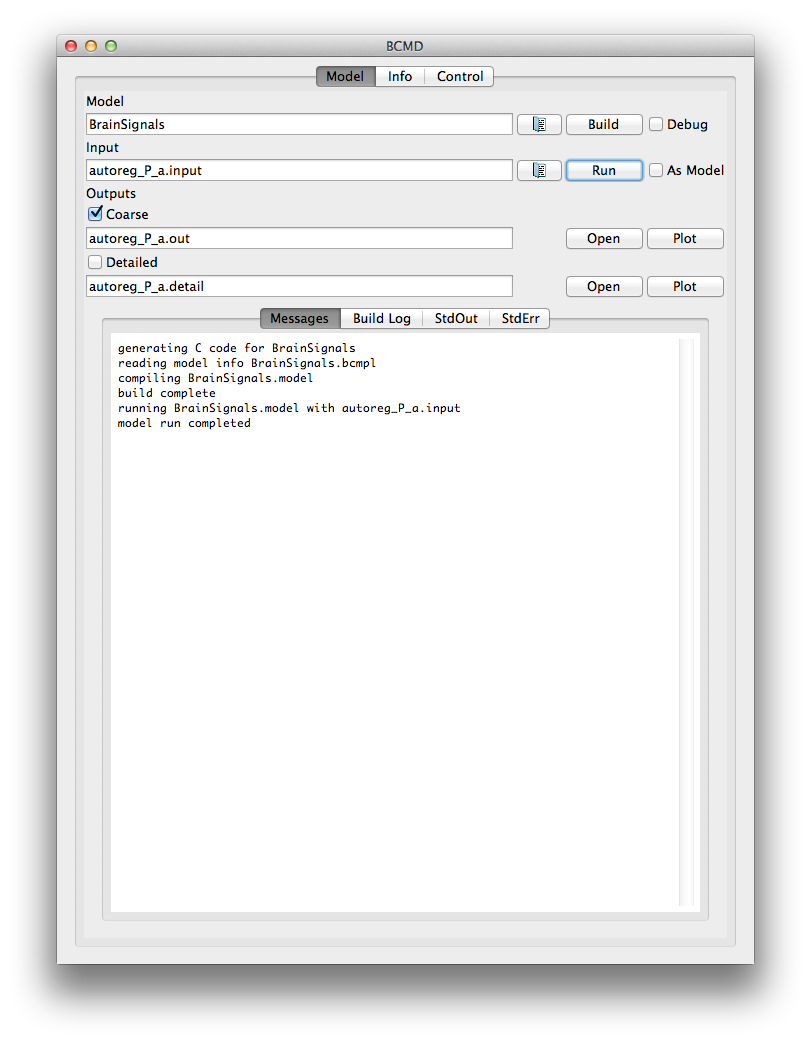
\includegraphics[scale=0.5]{figures/mainwindow.png}
\caption{BGUI main interface window}
\label{fig:bgui:main}
\end{center}
\end{figure}

\subsection{BGUI}\label{bgui}

BGUI is a work-in-progress graphical interface for building models and running them with a chosen input file. It provides limited facilities for viewing and plotting the results, though these are mostly useful as an immediate sanity check---more quantitative analysis should be done in a proper numerical environment like R or Matlab. It can also display information about models and provides tools to help with construction of the input files that control a model run.

Use of BGUI requires the Python graphical interface toolkit Tkinter, along with the Matplotlib plotting library and the NumPy \& SciPy mathematics packages. Generation of model dependency graphs requires the GraphViz tools.

BGUI is launched from the command line like this:
\begin{verbatim}
    python bgui.py
\end{verbatim}
(On Unix platforms the script is executable, and may be invoked directly. However, explicitly including \texttt{python} is more dependable.)

A number of program settings, such as the current model and input file, are saved to a preferences file and reloaded when BGUI is launched. This \textit{shouldn't} cause problems, but if you encounter any issues it may be worth deleting this file, which is named \texttt{.bcmd\_prefs} and saved in your user home directory.

The main BGUI window is shown in Figure \ref{fig:bgui:main}. (The exact appearance will vary from platform to platform). It has a tabbed interface whose three tab panels, \textbf{Model}, \textbf{Info} and \textbf{Control}, are described in the sections below.

\subsubsection{Model Window}\label{bgui:model}
The area at the top controls the building and running of models. You can either specify a model by name or press the adjacent button (with the indecipherable blue icon) to bring up a file selection dialog to choose a \texttt{.modeldef} file. Once selected, press `Build' to build and compile the model. The checkbox at the right determines whether the model is built in debug mode.

Once a model has been built, you can run it with a specified input file. Again, click the adjacent blue button to choose the file, and then the `Run' button to run the model with it. (The checkbox on this line determines whether, when you choose a model file, the input file name should be updated to match. Although this may be marginally useful in some simple situations, it is rather non-obvious and will probably be changed in future.)

The next two rows specify whether to generate coarse and/or detailed outputs, and what the names of these files will be. The output names are automatically set to match the input file (and this will cascade from the model file if the 'As Model' checkbox is checked), but can be changed if desired.

The area at the bottom of the window contains several different log consoles, giving messages from different parts of the build and run process. The first, `Messages', gives short summary messages from BGUI itself. `Build Log' shows messages received while compiling the model, which may be useful if the build fails. `StdOut' and `StdErr' show the two output streams from running the model itself---the latter may be prohibitively large for a sizeable model in debug mode.

(Note that model definitions and input files may be located anywhere you like, provided that you use the file dialogs to specify them. If you type the names directly, BGUI will look for them in the last directory you specified for the corresponding file type. For the moment, build products such as the model executable itself and the resulting data files are always placed in the standard BCMD \texttt{build} directory---at some point there will probably be a way to change this.)

\begin{figure}[tbph]
\begin{center}
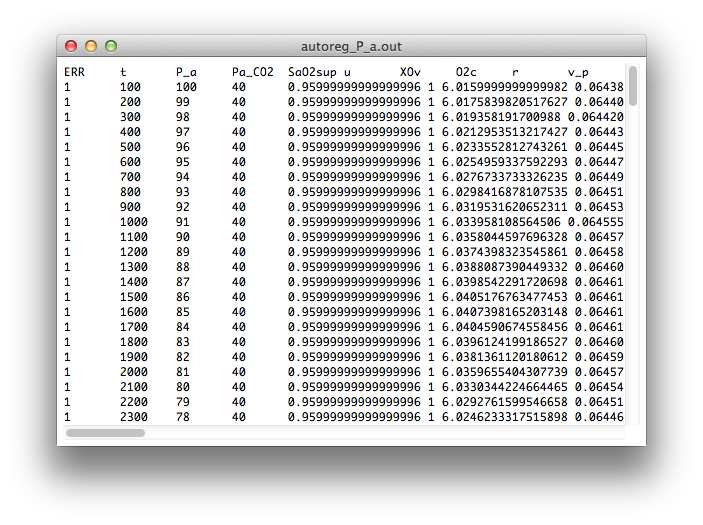
\includegraphics[scale=0.5]{figures/textout.png}
\caption{BGUI textual results display}
\label{fig:bgui:text}
\end{center}
\end{figure}

\begin{figure}[tbph]
\begin{center}
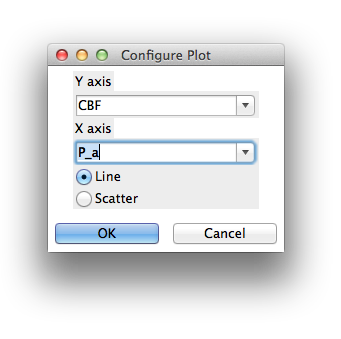
\includegraphics[scale=0.7]{figures/plot-select.png}
\caption{BGUI plot data selection dialog}
\label{fig:bgui:choose}
\end{center}
\end{figure}

\begin{figure}[tbph]
\begin{center}
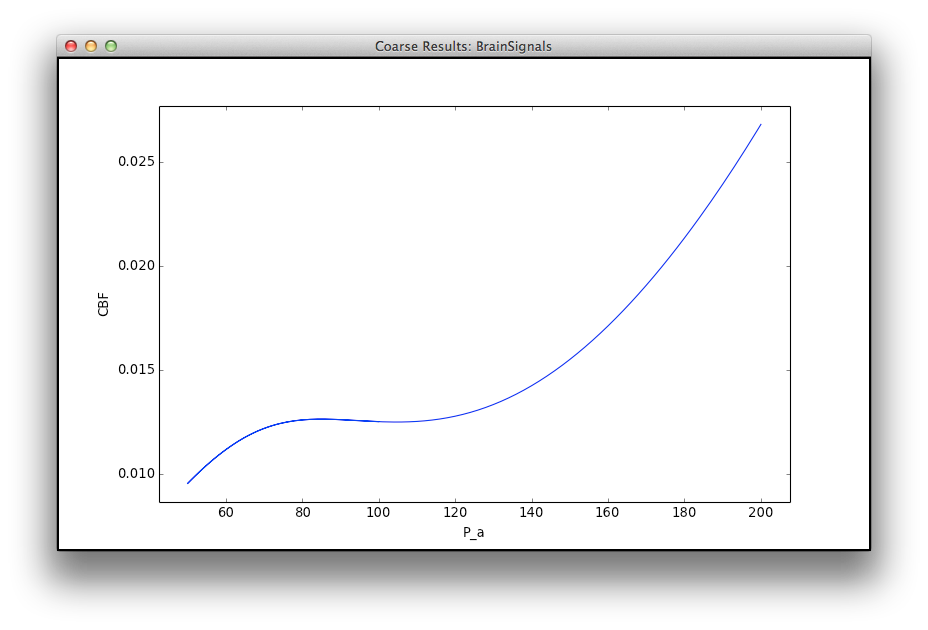
\includegraphics[scale=0.5]{figures/plot.png}
\caption{BGUI plot window}
\label{fig:bgui:plot}
\end{center}
\end{figure}

Once a model has been successfully run, you can examine the outputs using the buttons to the right of the respective output filename. The `Open' button will display the tab-delimited results in a simple text window (Figure \ref{fig:bgui:text}), while the `Plot' button allows simple plotting. It will first pop up a dialog (Figure \ref{fig:bgui:choose}) allowing you to select the plot type and which column from the result file should be plotted on each axis. (It is not currently possible to plot multiple traces together, nor to plot data directly from the input file.) Once you `OK' the configuration, the plot itself will appear (Figure \ref{fig:bgui:plot}). Note that both the text and plot windows are self-contained, so you can have several open at once, which is not as useful as plotting together but at least allows some comparisons to be made.

\begin{figure}[tbph]
\begin{center}
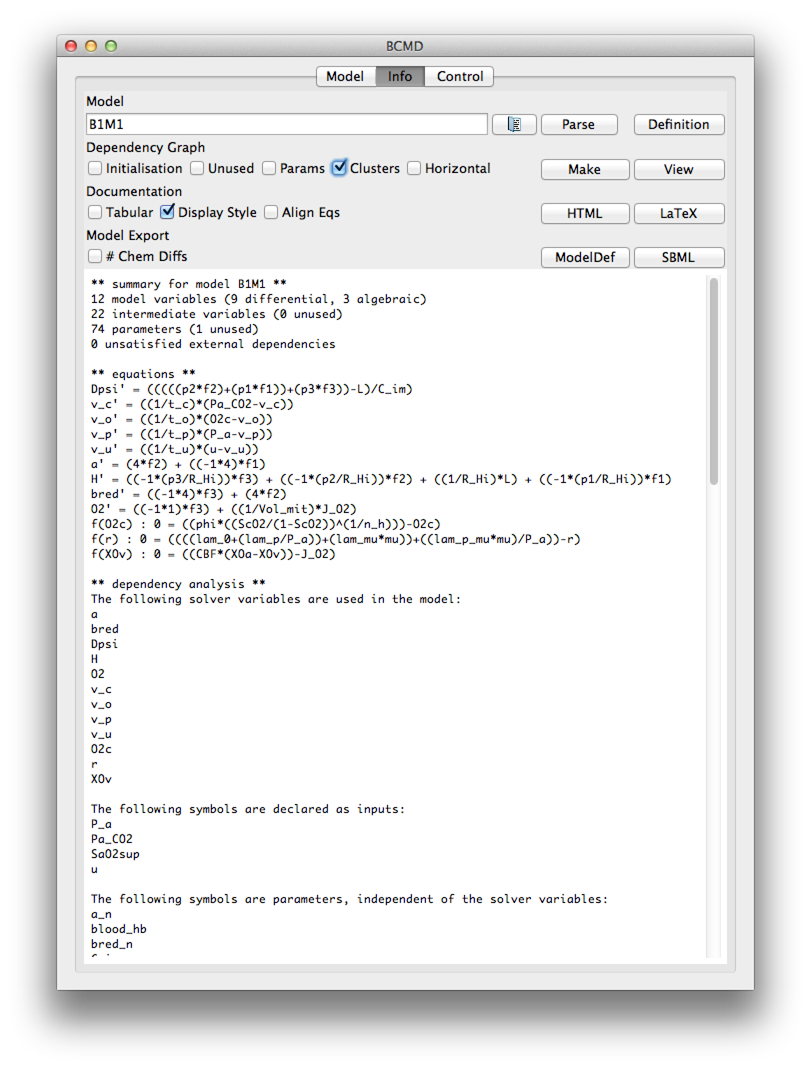
\includegraphics[scale=0.5]{figures/info.png}
\caption{BGUI info pane}
\label{fig:bgui:info}
\end{center}
\end{figure}

\subsubsection{Info Window}\label{bgui:info}

The Info window (Figure \ref{fig:bgui:info}), as the name suggests, provides information about the current model. Note that this is only up to date after the model has been successfully built. The bulk of the information is shown in the large text area that occupies most of the window. This includes summary data about the size of the model, a list of the model equations, some dependency analysis, etc.

The area at the top of the panel allows you to specify the current model, either by entering the name or using a file dialog. This is the same model as on the main Model window---selecting on either tab panel will also change the model on the other.

The `Parse' button reads the model information generated when the model was compiled. BGUI will do this automatically when it builds the model, so it is rarely necessary to use this button. However, if for some reason you want to load the info for a model without rebuilding it first, you can do so here, provided the model has been built previously and the resulting (\texttt{.bcmpl}) info file remains available. The `Definition' button will display the model definition itself in a simple text window. Note that this is not a proper text editor and you cannot save changes from here, it is only for viewing.

The next row allows you to configure and build a dependency graph like the one shown in Figure \ref{fig:graph}. The first four checkboxes specify whether the graph should include: symbols that are only used at initialisation; symbols that never feed back into the model behaviour (often representing output or measurement processes); parameters; and whether symbols should be clustered into subgraphs based on their tags (see \S\ref{info} and \S\ref{model:tags}). The fifth checkbox, `Horizontal', specifies the principal direction\footnote{In the absence of cycles, dependent nodes in the graph are positioned either below or to the right of nodes on which they depend. Even moderately complex models will often include cycles, which will break this ordering, but the overall direction is generally maintained. For example, the graph in Figure \ref{fig:graph} is drawn in top-to-bottom order.} of the graph: if checked, the graph is drawn from left to right, otherwise it is drawn from top to bottom.

Once the settings have been chosen, the `Make' button creates the graph in PDF and GIF formats---the files are saved in the usual \texttt{build} directory and have the same base filename as the model. The `View' button opens the generated GIF in its own window, but note that this viewing option is \textit{extremely} primitive. In particular, it does not support rescaling, so often only a small portion of the graph can be seen at a time. This is mainly intended for spot-checking that the graph creation worked---for proper examination, open the PDF version in a standard PDF viewer.

The Documentation controls in the next row allow you to generate model documentation. This is based on the model definition, supplemented with any information you have provided in documentation comments (see \S\ref{model:doc:comments}). The `HTML' button will generate documentation in HTML format, viewable in any reasonably up-to-date web browser. The generated file is named \textit{modelname}\texttt{.html}, and is created in the standard \texttt{build} directory. Similarly, the `LaTeX' button generates documentation in \LaTeX{} format, writing the results to \texttt{build/}\textit{modelname}\texttt{.tex}. The content of the files generated in the two formats is broadly equivalent, but they are not identical.

The HTML documentation is mostly intended for use as a reference by model developers. It includes a number of implementation details such as source model files, embedded code, symbol types and tag membership and also provides a lot of internal hyperlinks. Chemical reactions are \textit{not} included, and mathematical expressions are shown in the somewhat opaque form the parser produces, with a lot of defensive parentheses---no attempt is currently made to improve their readability, although this will likely be added in future. At present there are no configuration options provided for HTML documentation.

The \LaTeX{} output is aimed more for inclusion in written papers or published supplementary materials, and focuses on presenting formul\ae{} and parameters. The checkboxes to the left allow some configuration of the output, although you may well also require some \textit{post hoc} adjustment to make things like equations fit correctly on the page. The current \LaTeX{} options are:

\begin{adjustwidth}{0.8cm}{0.8cm}
\begin{description}
\item[Tabular] If this box is checked, variables and parameters are listed in a \texttt{longtable} environment; otherwise they are presented in a \texttt{description} list (like the one describing these options). The former may be more appropriate for some kinds of document, but it will usually require more fiddling with the generated \LaTeX{} code in order to make the columns look right on the page. The description format is less economical with space, but will probably need less manual intervention.
\item[Display Style] If this is checked, mathematical symbols and expressions are drawn in the `display' style, otherwise standard inline formatting is used. The latter makes somewhat better use of vertical space, and may lead to better arrangement of text on the page, but will often render complex expressions and fractions unreadably small. Since the generated documentation is mostly a bunch of lists or tables anyway, uniform body text is probably not a primary concern, so enabling display style is recommended.
\item[Align Eqs] If this is checked, the differential and algebraic equations in the model are rendered using an \texttt{align} environment, rather than as a sequence of separate \texttt{equation} environments. If your equations are all quite short, this \textit{may} look better---the principal difference is that all the equals signs should line up---but if there are long equations that you need to split across more than one line then it becomes quite inconvenient. For that situation, use the normal equation format, then edit the generated file to use a \texttt{split} environment for the problematic equations.
\end{description}
\end{adjustwidth}

The generated file is a complete \LaTeX{} document with a simple \texttt{article} wrapper that includes the necessary packages. It should be possible to typeset it directly. You can also easily copy out the bulk of the content into another document of your choice. Note that \texttt{ams math} package is required in all cases. In addition, the \texttt{mhchem} package is needed if there are any chemical reactions in the model, and the \texttt{longtable} package is required if you have exported using the `Tabular' option.

The Model Export controls allow you to export the model definition in two formats.

The `ModelDef' button saves the current model as a self-contained BCMD model definition file with standard formatting. This can be useful in cases where the model definition is spread across a number of different files, particularly if you wish to make the model available to someone else. If the model includes chemical reactions, they are included as such in the exported definition. However, it can be useful to see the differential equations that the compiler has constructed from the reactions. If the (admittedly cryptic) `\# Chem Diffs' checkbox is ticked, the exporter adds these differential equations \textit{as comments} in the relevant section of the modeldef file. The generated file is named \textit{modelname}\texttt{.modeldef}, and is created in the standard \texttt{build} directory. Be aware that if your original model definition is in this directory (this is not recommended, but possible), then using this export option will overwrite it.

The `SBML' button exports the model using the \href{http://sbml.org}{Systems Biology Markup Language} \citep{Hucka:2003fs,Finney:2003wp}. The generated file is named \textit{modelname}\texttt{.xml}, in the standard \texttt{build} directory. Note that this feature is \textit{extremely provisional}. Some BCMD features cannot be easily represented in SBML, and others sort-of can but aren't yet. Export results may not be valid SBML, or may not exactly reproduce the original model. Handle with care!

\subsubsection{Control Window}\label{bgui:control}

The Control window (Figure \ref{fig:bgui:init}) provides tools for creating BCMD input files, including explicit parameter setting, data import and/or synthesis and choice of outputs.

The region at the top of the window is used to specify the file to be created. Enter the intended filename in the `File' field. The button with the indecipherable blue icon is in this case used to choose the \textit{directory} in which to create the named file, rather than the filename itself (since the file may not exist yet). Once the file has been identified, the `Generate' button will create the file. (Pressing `Return' or `Enter' after entering text in the filename field has the same effect as pressing this button.) If the `Set Input' checkbox is ticked, then generating the input file will set the generated file as the current input file in the Model window. If the `Run' checkbox is also ticked, the model will then be automatically run with that input. (If `Set Input' is not checked, the `Run' setting is ignored.)

The contents of the generated file are specified in the tabbed region below. There are three separate tabs, corresponding to different conceptual stages of running the model: initialisation, the actual simulation steps, and output generation. These are described in the following sections.

Note that a standard simulation workflow is assumed. Some of the more esoteric capabilities of the input file format---such as sending different data to the coarse and detail output streams, or emitting headers somewhere other than at the top of the file---are not supported here. However, the omitted features are seldom used in practice. 

\begin{figure}[tbph]
\begin{center}
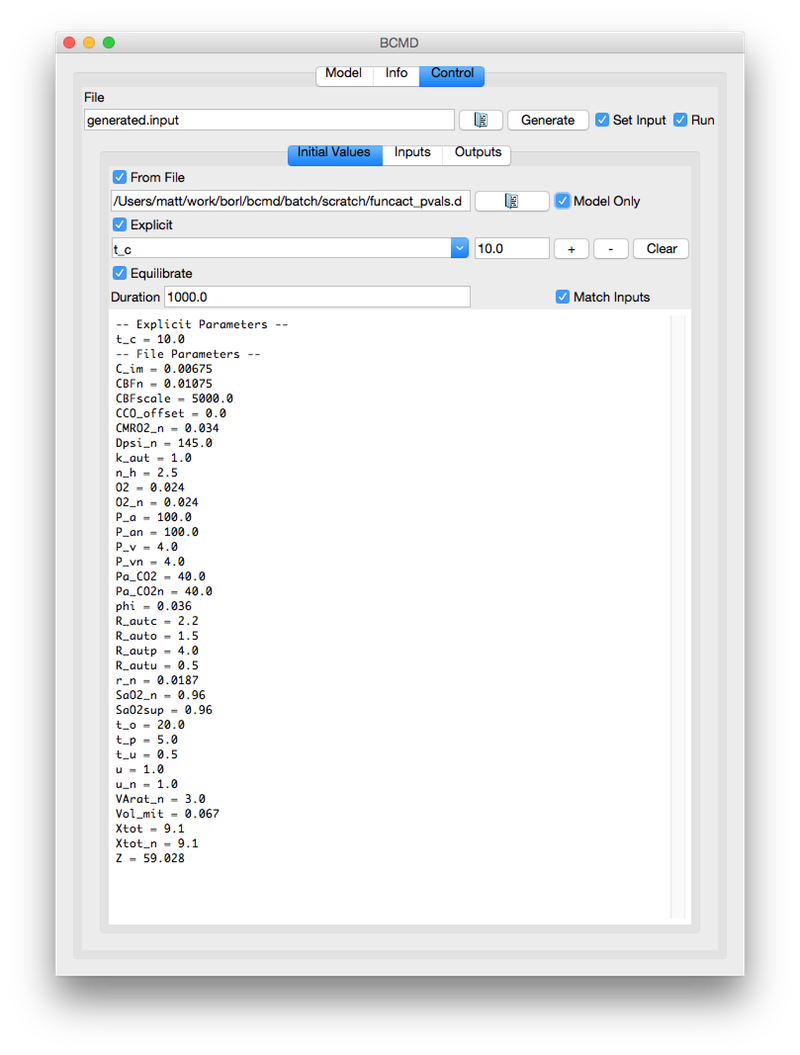
\includegraphics[scale=0.5]{figures/init.png}
\caption{BGUI control/initial values pane}
\label{fig:bgui:init}
\end{center}
\end{figure}

\subsubsection{Initial Values}\label{bgui:init}

The Initial Values panel  (Figure \ref{fig:bgui:init}) allows the values of model parameters and variables to be set prior to beginning the simulation, and also supports an optional initial equilibration period to allow the values to `burn in'. Values may be specified individually and/or imported wholesale from a file.

If the `From File' checkbox is ticked, parameter values will be loaded from the file specified in the associated text field. Use the icon button to select the file via a standard open file dialog. Supported file types are comma-separated value (\texttt{.csv}), tab-delimited text (\texttt{.txt}) and the old BRAINCIRC (\texttt{.dat}) format. For text and CSV, the values can be arranged by rows or by column. Only numeric values can be assigned---any other values in the file will be ignored.

If the `Explicit' checkbox is ticked, values may be specified manually. The name of the parameter to be assigned can be typed into the associated combo box control (shown containing `t\_c' in the figure), or selected from the box's popup menu, which should list all of the symbols in the current model (assuming it has already been built). Enter the value for the parameter in the adjacent text field (containing 10.0 in the figure) and press the `+' button to add it to the list of initial values shown below. The `--' button removes the specified parameter from the explicit assignments, while the `Clear' button erases all explicit assignments. (Note that when a parameter is set explicitly that also appears in the parameter file, the explicit value takes precedence.)

The `Model Only' checkbox specifies whether variable and parameter names that are not present in the current model should be included in the generated input file. It may be useful to uncheck this if you wish to generate a file that will be used with several different models with different sets of parameters.

To run the model for a period before beginning the simulation proper, check the `Equilibrate' checkbox. The length of this equilibration period is specified in the `Duration' field, in whatever time units the model uses (typically seconds).

The `Match Inputs' checkbox specifies that initial values should be provided for any variables and parameters for which there are input signals (see below), such that their value prior to the simulation is the same as the value they are given in the first simulation step. This is useful to avoid an initial transient when the simulation begins, especially if you are equilibrating. (This only applies for symbols for which you have not specified an explicit value in this section. Explicit values always take precedence. Input matching will, however, override values loaded from a parameter file.)

The large text area at the bottom of the panel lists all initialisations that will be included in the generated file. It \textit{should} update as you make changes, although there might be a few edge cases where the updating does not happen immediately.

\begin{figure}[tbph]
\begin{center}
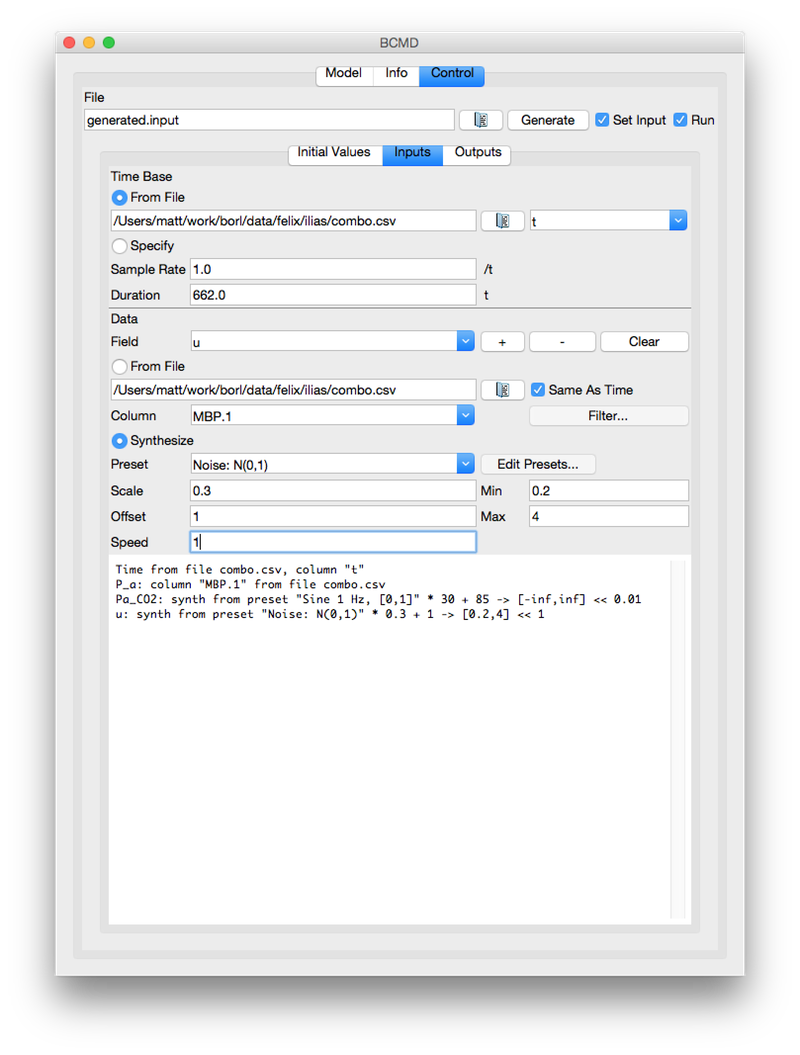
\includegraphics[scale=0.5]{figures/inputs.png}
\caption{BGUI control/inputs pane}
\label{fig:bgui:inputs}
\end{center}
\end{figure}

\subsubsection{Inputs}\label{bgui:inputs}

The Inputs panel (Figure \ref{fig:bgui:inputs}) specifies the actual time steps of the simulation. At present, only a single step sequence is supported---it is not possible to chain together data from different sources in succession, or have different sets of parameters set at different stages. So for more complex simulations it may be necessary to concatenate data files externally before importing. However, many basic cases are catered for.

The upper portion of the panel concerns the `Time Base' for the simulation---i.e., the actual time points over which the model is evaluated. These may either be imported from an external file---for example, containing real experimental data---or synthesised. The two radio buttons in this section determine which of those options is used.

If `From File' is selected, then the time base is imported from the file specified in the field below. Use the button with blue file icon button to choose a file---supported file types are CSV and tab-delimited text. When a valid file is chosen, the names of the columns of data in the file are loaded into the combo box control to the right. Use this to choose which column contains the time data. (At some point this may be updated to make an educated guess from the column names, but for the moment you need to choose explicitly even if the file contains only one column called `t` or whatever.)

If the `Specify' button is selected instead, then the time base will be generated from the values given in the `Sample Rate' and `Duration' fields. The generated time base always starts from time 0, and the units are whatever the model is defined with.

The central portion of the panel concerns the parameter settings that occur at each time step. As with the time base, these may either be drawn from an external file or synthesised in a number of preset forms. In either case, the field in question must first be chosen using the `Field' combo box, either by selecting from the pop up menu of model symbols, or by typing any valid identifier of your choice. (You can use a name not in the current model if desired---this may be useful if the same input file will be used with several different models.) The `+' button adds the field to the set that will be included in the generated file---using whatever form has been defined in the sections below. Note that the settings are captured at the point you add them---if you wish to alter the parameters for the signal, you must press `+' again after having done so. The `--' button removes the chosen field, while `Clear' removes all fields.

If the `From File' radio button is selected here, the sequence of values for the chosen field will be imported from a file, in the same way as the time base; again, CSV and tab-delimited text are supported. Note that the values for different fields can be drawn from different files, depending on the setting in the `Same As Time' checkbox: if this is ticked, then a single file is shared for everything---time base and \textit{all} file-based fields. In that case, a file chosen via the selection dialog in either section will immediately apply to both. Conversely, if `Same As Time' is unchecked, then every field retains its own file source, which can only be changed by re-adding the field using the `+' button. Either way, you must choose which column in the file to use for the field using the `Column' combo box below.

(The `Filter...' button is intended for post-processing the imported data. At present, though we have the functionality to do this, there is no user interface to do so. This will be added soon, but in the meantime this button is disabled.)

If the `Synthesize' radio button is selected, the values to be set are instead generated artificially according to a signal `Preset', chosen from the pop up menu. Several simple presets are currently supplied:

\begin{adjustwidth}{0.8cm}{0.8cm}
\begin{description}
\item[Noise: N(0,1)] Gaussian noise with mean 0 and standard deviation 1.
\item[Noise: U(0,1)] Uniformly-distributed noise on the interval [0,1].
\item[Random Walk] A drifting baseline generated as the cumulative sum of Gaussian noise with mean 0 and standard deviation 0.1.
\item[Sine 1 Hz, {[0,1]}] A standard sinusoidal wave at 1 Hz, scaled into the interval [0,1].
\item[Saw 1 Hz, {[0,1]}] A sawtooth wave rising from 0 to 1 at 1 Hz.
\item[Square 1 Hz, {[0,1]}] A square wave (50\% duty cycle) with frequency 1 Hz and off and on values 0 and 1 respectively.
\item[NIRS mix, {[0,1]}] A mixture of four sinusoids at different frequencies, with added Gaussian noise, scaled into the interval [0,1]. (Based on the simulated signal in \citet{Scholkmann:2010iy}.)
\end{description}
\end{adjustwidth}

(Again, much of the functionality for user-definable presets has been implemented, but this requires a pretty complicated UI that doesn't yet exist, so the corresponding button is disabled for the moment.)

Presets can be adapted somewhat using the settings below:

\begin{adjustwidth}{0.8cm}{0.8cm}
\begin{description}
\item[Scale] Specifies a value by which the synthetic signal should be multiplied. (Default: 1)
\item[Offset] Specifies a value to be added to the signal. (Default: 0)
\item[Min] Specifies a lower bound at which signal values should be clamped. (Default: $-\infty$, i.e. unbounded below)
\item[Max] Specifies an upper bound at which signal values should be clamped. (Default: $\infty$, i.e. unbounded above)
\item[Speed] Specifies a multiplier for the time base (or, equivalently, frequency) of the signal. Low values decrease the frequency, high values increase it. This has no effect on the noise presets, since those are time-independent. (Default: 1)
\end{description}
\end{adjustwidth}

The text area at the bottom of the panel gives a summary of all the selected inputs in a brief shorthand form. See Figure \ref{fig:bgui:inputs} for examples.

\begin{figure}[tbph]
\begin{center}
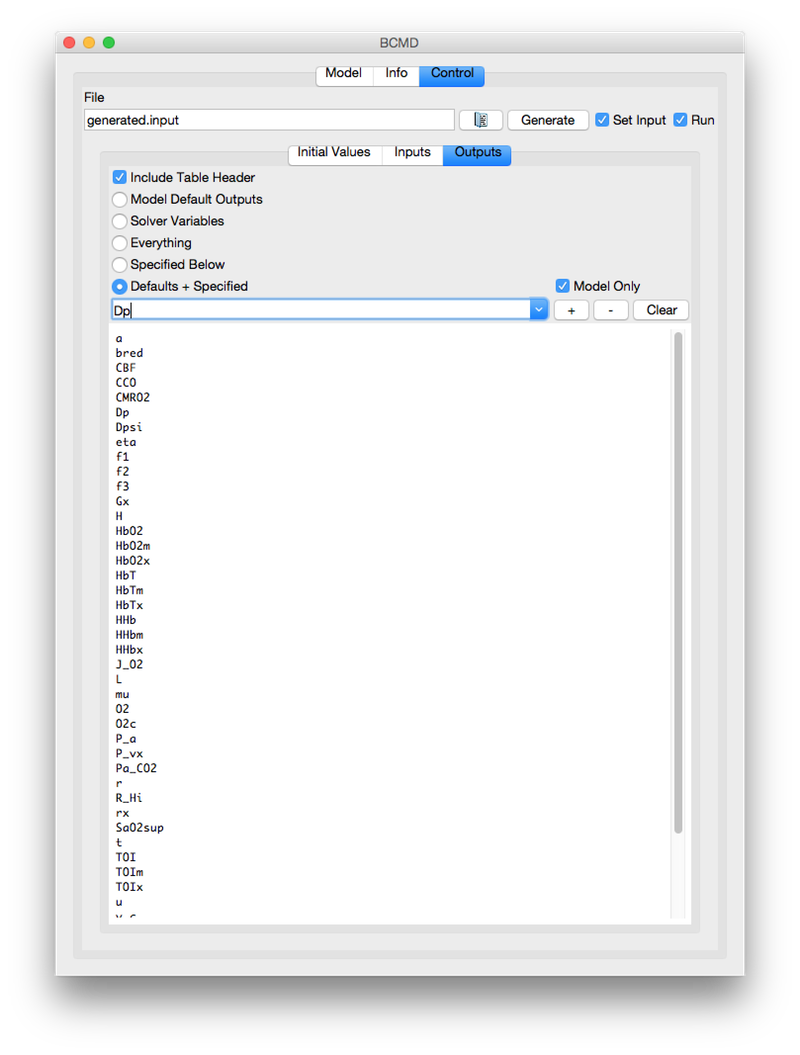
\includegraphics[scale=0.5]{figures/outputs.png}
\caption{BGUI control/outputs pane}
\label{fig:bgui:outputs}
\end{center}
\end{figure}

\subsubsection{Outputs}\label{bgui:outputs}

The Outputs panel (Figure \ref{fig:bgui:outputs}) controls what will be included in the output data generated when the simulation runs. The same set of fields is used for both coarse and detailed results (see \S\ref{runtime} for an explanation of the difference).

The `Include Table Header' checkbox, as the name suggests, specifies whether the output files should include a header row giving the names of parameters reported in the corresponding column of the output. This is usually a good idea unless the output is going to be passed to some existing process that does not understand such headers.

The radio buttons below provide a number of different output options:

\begin{adjustwidth}{0.8cm}{0.8cm}
\begin{description}
\item[Model Default Outputs] Do not specify any particular output fields, but instead tell the model to output whatever have been defined as the default output fields within the model itself.
\item[Solver Variables] Include only the variables that are actually solved, i.e. those in the \textbf{y} vector in Equation \ref{eq:general}. If nothing else has been specified in the model, this will be equivalent to the default outputs, but note that with this option the field list is included explicitly rather than being left up to the model.
\item[Everything] Include \textit{all} symbols that are defined in the model. This can result in very large output files, and often also highly redundant since many parameters will not change during a simulation. However, it can be useful for debugging purposes. Again, the field names are included explicitly in the generated file, as derived from the current model.
\item[Specified Below] Explicitly choose the fields to be exported, using the combo controls below.
\item[Defaults + Specified] As above, but the default outputs of the current model are added to the explicit list automatically.
\end{description}
\end{adjustwidth}

Assuming the current model has been successfully built, all symbols from the current model will be listed in the combo box popup menu below. You can also type any other (syntactically valid) name of your choice, although obviously the model will be unable to output fields it does not contain. Press the `+' button to add the chosen field to the list of outputs, or the `--' button to remove it. The `Clear' button will remove all explicitly-specified output fields (but not those inherited from one of the other options).

The `Model Only' checkbox specifies that only field names that actually exist in the current model should be included as outputs in the generated file. Again, this depends on the current model having already been built.

The complete list of fields that will be output is shown in the text area at the bottom of the panel. (Note that in the case of `Model Default Outputs' this list is implicit, and may vary if the model definition changes or if the file is used with a different model.)

\subsection{Batch processing tools}\label{batch}

Our computational experiments often involve running large numbers of model simulations under varying conditions. Several scripts used for this purpose can be found in the \texttt{batch} subdirectory of the BCMD distribution. Note that these are still very much works in progress, often unfriendly and in some cases undocumented. The current implementations are pretty \textit{ad hoc} and will likely be rationalised in future.

There are two main scripts: \texttt{dsim.py} (\S\ref{batch:dsim}) manages the running of deterministic or quasi-determ\-inistic batches of simulations, primarily (so far) for the purposes of sensitivity analysis, while \texttt{optim.py} (\S\ref{batch:optim}) performs parameter estimation by traditional optimisation\footnote{A third script, \texttt{abcmd.py}, attempts to do parameter estimation via Approximate Bayesian Computation. At present this is not functioning correctly and is not documented here.}. The scripts make use of a plain text \textit{job file} to define the batch task to be performed---these vary between the scripts, but share the same overall format and many common features---these are described in \S\ref{batch:common}.

The batch tools are run from the command-line. They are unlikely ever to have a GUI in their own right---batch processes are inherently non-interactive---but some tools for constructing the input and job files \textit{may} be added to BGUI eventually.

If the facilities described here don't fit your needs, it may be possible to write a simple wrapper script in Python (or possibly some other language you are happy with) to do what you require. Some fairly trivial examples are included in the \texttt{batch} directory. These are not documented---they are just `quick \& dirty' hacks to run some jobs that we needed at some point---but may provide a useful starting point. E.g., have a look at \texttt{co2batch.py}, a simple hard-coded batch script that runs a sequence of \texttt{dsim} jobs over a directory of data sets.


\subsubsection{Shared Features}\label{batch:common}

All three main batch scripts take two arguments, like this:
\begin{verbatim}
      python script.py jobfile datafile
\end{verbatim}
The job file specifies details such as what model to use and what variables to simulate, while the data file specifies time series data that will be used when running the job. The latter should be a CSV or tab-delimited text file, with column headers that will be used to identify the variables or inputs. (It is also possible to use a BRAINCIRC \texttt{.dat} file as the data source, but hopefully the necessity for that is asymptoting to zero...)

Job files are line-oriented plain text. Blank lines, lines starting with a hash character \texttt{\#} and lines specifying any details the script doesn't recognise are simply ignored. Lines defining the job start with a keyword, followed by a colon, then one or more details, separated by commas, as in the following snippet:
\begin{verbatim}
      # specify which model to use
      model: BrainSignals
      
      # variable to be simulated
      # with the distribution of initial conditions
      var: CBF, constant, 0.01075
\end{verbatim}

Several fields, like \texttt{var} in the above example, allow a \textit{distribution} to be specified. How (or whether) this is actually used varies according to context. The first element (following the variable of parameter name) is the distribution type, followed by some optional parameters (all of which default to 0) and an optional default value (which may be calculated from the parameters if they are given and it isn't). Four types are recognised:
\begin{adjustwidth}{0.8cm}{0.8cm}
\begin{description}
\item[constant, {[\textit{value}]}] No variation, always use the specified value, or 0 if omitted.
\item[uniform, {\textit{min}, \textit{max} [, \textit{default}]}] The value is uniformly distributed between \textit{min} and \textit{max}. The default default is $(min + max)/2$.
\item[normal, {\textit{mean}, \textit{variance} [, \textit{default}]}] The value is normally distributed with specified mean and variance. Default defaults to \textit{mean}.
\item[lognormal, {\textit{mean}, \textit{variance} [, \textit{default}]}] Value follows a log-normal distribution, where the underlying normal distribution has the specified mean and variance. Default defaults to $e^{mean}$.
\end{description}
\end{adjustwidth}
Any distribution that is not otherwise specified defaults to \texttt{constant, 0}.

While each kind of job has some keywords that are specific to it, the following are used by all three scripts:

\begin{adjustwidth}{0.8cm}{0.8cm}
\begin{description}
\item[model] Name of the model to be used for the simulations. This should be just the name itself, without any file extensions, and should follow the rules for model identifiers (numbers, letters and underscores, not starting with a number). Various other job details are constructed from this if they are not independently specified.
\item[var$^{\dagger}$] An output to be simulated in the model. The first element is the name of the variable. A distribution can be specified in subsequent elements---if the job type supports it, this is used for drawing the initial value of the variable at the start of the simulation. A target time series for the variable should usually be provided in the input data file (possibly aliased, see below), although in some cases it is possible not to do so (in which case the results will be evaluated relative to 0).
\item[input$^{\dagger}$] An input for which time series data will be supplied to the model. Data must be provided in the input data file (possibly aliased, see below). The first element is the name of the input parameter or variable. Optional subsequent elements specify its distribution---if the job type supports it, this is used to \textit{perturb} the supplied data (i.e., to add noise so that the inputs are not identical each time).
\item[param$^{\dagger}$] A parameter that can be set in the simulation. The first element specifies the parameter name. Optional subsequent elements specify a distribution, which is used in different ways by the different job types. Note that parameters can be described and then not used---see \texttt{param\_select} below.
\item[param\_file$^{\dagger}$] Specify an optional external file containing parameter details. This can be useful if you have a lot of parameters with the same distributions used in different jobs. The file can be a CSV or TXT file, but is treated in a line-oriented rather than tabular fashion (so different rows need not have matching columns). Each row is interpreted as if it were the right hand side of a \texttt{param} entry in the job file, i.e. the parameter name followed by an optional distribution. If a parameter in this file is also explicitly specified in the job file, the job file version overrides the settings in the parameter file.
\item[param\_select$^{\dagger}$] Specify the parameters that will actually be used in the job. Each element on the right hand side is a parameter name. If this keyword is not present, or if any element is an asterisk \texttt{*}, then all parameters for which a distribution has been specified, in both the job file and the parameter file, are included.
\item[alias$^{\dagger}$] Specify that an input or variable time series appears in the input data file under a different name. The first element is the name in the model, the second is the name in the file. If not specified, variables are assumed to have the same name in both, with one exception:

\textbf{IMPORTANT:} For historical reasons involving the support of BRAINCIRC files, internal processing of the independent variable (usually time) in these scripts uses a different proxy name. If you explicitly specify times in your input data file (almost always the right thing to do), you need to include an alias for it \textit{even if it seems to have the right name already}. Use a line like this:
\begin{verbatim}
      alias: t, t
\end{verbatim}
Yes, this is obviously stupid. It will probably be sorted out in future, but for now just go with it.
\item[program] The model executable. Defaults to \texttt{build/}\textit{modelname}\texttt{.model}. You should only need to specify this if you're doing something unusual.
\item[work] Name of a directory in which to place work and result files. The given directory is created inside the standard \texttt{build} directory. If not specified, a new directory is created at \texttt{build/}\textit{modelname/timestamp}.
\item[model\_io] Name of a directory in which to place the simulation input and output files. This directory is placed inside the work directory, above. By default it is called \texttt{model\_io}.
\item[init] Specifies a BCMD or BRAINCIRC input file to use as the initial steps of every simulation in the batch. This sequence is simply prepended to the generated one---this means the steps are executed \textit{before} any parameter setting specific to the batch job is performed.
\end{description}
\end{adjustwidth}

Any keyword can occur multiple times in the job file without error. Those marked above with a $\dagger$ symbol are \textit{intended} to support multiple occurrences, and all specified values are used---clearly it may be necessary to simulate more than one output or vary more than one parameter. For the remaining, unmarked, keywords, only the first occurrence is used---subsequent appearances are legal but ignored.

All the batch processing scripts depend on the \texttt{model\_bcmd.py} module, which implements a class conforming to the ABC-SysBio model interface. This wraps up the process of invoking a BCMD model with given inputs, and then reading and returning the results. It also handles parallelisation, allowing it to run some specified number of models simultaneously, which should be faster on multi-core systems (this is only supported for \texttt{dsim} and \texttt{abcmd} at present, not for \texttt{optim}).

Most of the business of constructing the step sequences for the model input files is handled by the \texttt{steps.py} module, which can also be invoked from the command line to help when constructing inputs of your own (see \S\ref{steps:py}). Reading data from TXT, CSV and BRAINCIRC files is handled using the \texttt{inputs.py} module. Some other data conversion utilities are \texttt{descs2csv.py} and \texttt{dat2csv.py}.

Finally, the \texttt{distance.py} module provides a number of distance metrics (or quasi-metrics), each in two forms, one conforming to an ABC-SysBio interface and the other in a simpler functional form. Each calculates a scalar value that in some way quantifies the distance between two vectors of the same length, say $\vv{a}, \vv{b} \in \mathbb{R}^N$. The following measures are currently supported:
\begin{adjustwidth}{0.8cm}{0.8cm}
\begin{description}
\item[euclidean] The Euclidean or $L^2$ distance is the most common distance metric, calculated as:
$$\text{euclidean}(\vv{a}, \vv{b}) = \left\| \vv{a} - \vv{b} \right\| = \sqrt{\sum_i a_i^2 - b_i^2}$$
\item[manhattan] The Manhattan, taxicab or $L^1$ distance is the sum of the absolute component differences:
$$\text{manhattan}(\vv{a}, \vv{b}) = \left\| \vv{a} - \vv{b} \right\|_1 = \sum_i \left| a_i - b_i \right| $$
\item[mean] The mean or RMS distance is the mean squared componentwise difference between the vectors:
$$\text{mean}(\vv{a}, \vv{b}) = \sqrt{\frac{\sum_i a_i^2 - b_i^2}{N}}$$
(This is literally just a scaled version of the Euclidean distance, but it's kept around for historical reasons.)
\item[loglik] The log-likelihood distance is based on the probability that the difference between the two vectors is attributable to Gaussian noise with some specified standard deviation, $\sigma$ (by default 1):
$$\text{loglik}(\vv{a}, \vv{b}) = \frac{N}{\sqrt{2\pi\sigma^2}} - \sum_i \frac{a_i^2 - b_i^2}{2\sigma^2}$$
\item[cosine] The cosine distance gives the cosine of the angle between the two vectors:
$$\text{cosine}(\vv{a}, \vv{b}) = \frac{1}{2} - \frac{\vv{a} \cdot \vv{b}}{2 \left\| \vv{a} \right\| \left\| \vv{b} \right\|}$$
(The factor of $\frac{1}{2}$ scales the result into the range {[0,1]}.)
\item[angular] The angular distance gives the angle between the two vectors:
$$\text{angular}(\vv{a}, \vv{b}) = \frac{1}{\pi} \arccos \left( \frac{\vv{a} \cdot \vv{b}}{\left\| \vv{a} \right\| \left\| \vv{b} \right\|} \right)$$
(The factor of $\frac{1}{\pi}$ scales the result into the range {[0,1]}.)
\end{description}
\end{adjustwidth}

\subsubsection{Deterministic Batches \& Sensitivity Analysis}\label{batch:dsim}

The \texttt{dsim.py} script runs multiple simulations with different combinations of parameter values, where the values are drawn from a set of defined `levels' according to a predefined scheme. This is nominally `deterministic' because the sequence of simulations is fully determined before any runs take place and does not change according to the results of individual simulations. Some job modes are indeed wholly deterministic and will run identically each time. However, in probably the most common usage, that of Morris-style trajectories for sensitivity analysis, there is nevertheless an element of randomness. It is also possible to add random perturbations to the input data.

The script is run with Python from the Unix or MSYS command line:
\begin{verbatim}
      python dsim.py [options] jobfile datafile
\end{verbatim}
(On Unix platforms the script is executable, and can probably be run directly. However, explicitly including \texttt{python} is more dependable.)

The following command line options are available:
\begin{adjustwidth}{0.8cm}{0.8cm}
\begin{description}
\item[-h, -{}-help] Print a usage message and exit.
\item[-{}-version] Print the program's version number and exit.
\item[-r FILE, -{}-results FILE] Specify a name for the output file. By default, the file is named \texttt{results.txt}.
\item[-s FILE, -{}-sensitivities FILE] Specify a name for the sensitivities file. By default, the file is named \texttt{sensitivities.txt}.
\item[-b DIR, -{}-build DIR] Specify the location of the build directory (this is where the model executable is expected to be). The standard BCMD \texttt{build} directory is used by default.
\item[-o DIR, -{}-outdir DIR] Specify a directory for working files and results. The default is a directory \textit{modelname}\texttt{/}\textit{timestamp} inside the specified build directory.
\item[-p, -{}-perturb] Enable perturbation of the input data (see below).
\item[-d, -{}-dryrun] Assemble the data and construct the set of jobs, then write all the configuration details to \texttt{stdout} and exit without simulating.
\end{description}
\end{adjustwidth}

The job files for \texttt{dsim} are conventionally given the file extension \texttt{.dsimjob}, although this is not enforced. In addition to the common features described \S\ref{batch:common}, the following keywords are supported:
\begin{adjustwidth}{0.8cm}{0.8cm}
\begin{description}
\item[job\_mode] What kind of job to run. This should be one of:
	\begin{itemize}
	\item \texttt{single}: Each selected parameter is varied across its range individually, while all other selected parameters are kept at their default value. Scales $\mathbf{O}(np)$, for $p$ parameters and $n$ levels.
	\item \texttt{pairwise}: Each pair of selected parameters is varied jointly across their ranges while all other selected parameters are kept at their default. Scales $\mathbf{O}(n^2p^2)$, for $p$ parameters and $n$ levels.
	\item \texttt{cartesian}: All selected parameters are varied jointly. That is, every possible combination of the available levels of all parameters is tried. Scales $\mathbf{O}(n^{p})$, for $p$ parameters and $n$ levels.
	\item \texttt{morris}: All parameters are varied by single steps in random sequence. This is an implementation of the Morris 'elementary effects' sampling scheme for sensitivity analysis \citep{Morris:1991vs,Campolongo:2007cv}. A single `trajectory' (of $p+1$ steps) samples sequential changes to all parameters. Construction of the trajectories is now delegated to the SALib library, as is analysis of the results. Scales $\mathbf{O}(kp)$, for $p$ parameters and $k$ trajectories.
	\item \texttt{fast}: Parameters are varied jointly along oscillatory trajectories with disjoint frequencies in each dimension. This is used for FAST sensitivity analysis \citep{Saltelli:1999ur}. Trajectory construction and analysis are performed using the SALib library. Scales $\mathbf{O}(kp)$, for $p$ parameters and $k$ samples.
	\end{itemize}
(Default: \texttt{single})
\item[divisions] The number of levels into which the parameter range should be divided. Simulated values are drawn from these discrete levels. Division is performed in \textit{quantiles} of the distribution specified for the parameter. In most cases you will probably want to specify a \texttt{uniform} distribution, in which case all levels are equidistant. For \texttt{normal} and \texttt{lognormal} distributions, steps close to the mean are closer together. (Both these distributions have infinite support, so obviously we don't span the whole range---instead, the range is divided into $divisions+2$ quantiles and the non-finite endpoints discarded.) Parameters specified as \texttt{constant} are not divided. This setting is ignored for \texttt{fast} jobs. (Default: 10)
\item[nbatch] The number of model instances than can be run in parallel. This is not guaranteed to make things faster, but may do so, especially for processor-bound jobs on multicore hardware. Try setting this to the number of cores in your machine. (Default: 1)
\item[beta] The number of repetitions of each job to run. This is ignored unless input perturbation was enabled when \texttt{dsim} was launched. With perturbation, it may make sense to run repeat simulations, since the runs will be non-identical. (Default: 1)
\item[timeout] Maximum time in seconds to allow an individual simulation to run before forcibly terminating it. While model runs are typically fast, there can sometimes be regions of the parameter space that lead the solver to get stuck for long periods, perhaps indefinitely. Such cases make the whole batch unacceptably slow, so after awhile we abandon the attempt. (Default: 30)
\item[npath] The number of Morris trajectories or FAST samples to run. Ignored for other job types. (Default: 10)
\item[jump] The number of levels to change parameters by during a Morris trajectory. Ignored for other job types. (Default: 4)
\item[interference] The interference factor, $M$, for FAST jobs. Ignored for other job types. (Default: 4)
\item[substitute] A value to be returned by the distance functions for simulations containing NaNs. This must be a valid floating point value. Sensible sensitivities cannot be calculated for failed outputs, so in some cases it may be desirable to either penalise them with a very large distance value, or ignore them by setting this to 0. However, either policy amounts to a dodgy hack, so use with care. If possible, it is better to adjust parameter ranges so valid outputs are produced. (Default: NaN values are returned when they occur)
\item[save\_interval] Since \texttt{dsim} batches can take a long time, we may want to save intermediate results as we go along. On the other hand, saving itself takes time, so doing it very often will just slow things down even more. This setting specifies how many batches (sets of \texttt{nbatch} parallel simulations) to run between each save. Set to 0 for no intermediate saves. (Default: 100)
\end{description}
\end{adjustwidth}
All these \texttt{dsim}-specific keywords are treated as single-valued: the first occurrence in the file is used, subsequent instances are ignored.

A \texttt{dsim} job may require very many simulation runs. As well as potentially taking a \textit{really} long time, simulation results are collated in RAM, so for very large batches the Python interpreter will eventually run out of memory. The order of complexity for each job mode is noted in the description above. Be especially wary of the exponential scaling of the \texttt{cartesian} mode---this can get out of hand very quickly. Avoid using \texttt{param\_select:*} in this mode for all but the tiniest models.

Simulation results are generated in a tab-delimited text file, by default called \texttt{results.txt}. The structure is straightforward but slightly opaque. The actual simulation data is in the lower right quadrant of the table. The top section contains information shared between all jobs, while the lower left quadrant specifies job details:
\begin{itemize}
\item The first column, \texttt{job}, specifies the simulation number. This starts at zero and increments for each new set of parameters to be simulated.
\item The second column, \texttt{rep}, specifies the repetition number of the job. This again starts at zero. It will only be non-zero if perturbation is enabled and \texttt{beta} $>1$ given in the job file.
\item The third column, \texttt{species}, identifies the output variable for which the row contains data.
\item The next $p$ columns give the values of all selected parameters in the job. These values will be identical in all rows for the same \texttt{job}. The column heading is the parameter name.
\item The remaining columns give the output value at each time point of the simulation. The column heading is the time point index, starting at zero, prefixed by \texttt{t}: \texttt{t0}, \texttt{t1}, \texttt{t2}...
\item The top row is a header specifying column names.
\item The next row gives values for the simulation independent variable, here always referred to as \texttt{t}. These are in the time point columns \texttt{t0}, \texttt{t1}, \texttt{t2}... The \texttt{species} column has the value \texttt{t}. All other columns contain the 'missing data' value \texttt{NA}.
\item The next few rows give the input signals shared by all jobs. The \texttt{species} column contains the input variable name, with the suffix \texttt{\_in} appended. The actual input values are in the time point columns \texttt{t0}, \texttt{t1}, \texttt{t2}...  All other columns contain the 'missing data' value \texttt{NA}.
\item The next few rows give the target output values for each output variable. The \texttt{species} column contains the output variable name, with the suffix \texttt{\_out} appended. The actual input values are in the time point columns \texttt{t0}, \texttt{t1}, \texttt{t2}...  All other columns contain the 'missing data' value \texttt{NA}.
\item The remaining rows report the actual simulation results for the specified \texttt{job}, \texttt{rep} and \texttt{species}.
\end{itemize}
In addition, some information about the job configuration is written to a file called \texttt{dsim.info}.

For Morris and FAST sensitivity jobs, an additional file is written, named \texttt{sensitivities.txt} by default. This contains the sensitivity results for each parameter. Once again, it is a tab-delimited text file. The first column gives the parameter names, while the remaining columns contain sensitivity measures for each output variable tested. Morris jobs generate four measures per signal (the mean, $\mu$, standard deviation, $\sigma$, the absolute mean, $\mu^{\star}$ and a 95\% confidence estimate of the `true' value of $\mu^{\star}$), while FAST jobs generate two (the first order sensitivity, $S_1$, and the total effect estimate, $S_T$). The columns are labelled accordingly.

\subsubsection*{Analysis}

The raw simulation data is useful, but often you just want to look at changes in the relationship of the generated signals to their target values. The script \texttt{postproc.py} computes a variety of distance metrics for each simulated output and also some summary statistics about them.

The script is invoked from the command-line like this:
\begin{verbatim}
      python postproc.py DIR
\end{verbatim}
(On Unix platforms the script is executable, and can probably be run directly. However, explicitly including \texttt{python} is more dependable.)

The script takes no optional arguments. The required argument \texttt{DIR} specifies the path to a directory that either contains \texttt{dsim} results itself, or else contains a number of subdirectories containing \texttt{dsim} results. In the latter case, it processes each such subdirectory separately. It does not recurse into lower level subdirectories, and it will skip any subdirectories that do not contain the expected result files.

\texttt{postproc} generates three output files:

\begin{itemize}
\item \texttt{brief.txt} contains some very minimal information extracted from the full \texttt{dsim.info} file. This is used by some other scripts, and also to quickly identify what's going on in the directory (since postprocessed directories typically all look the same). At present the only content is the name of the source data file that was used to drive the simulations.
\item \texttt{distances.txt} contains distance metrics for every output signal in the \texttt{results.txt} file. All six of the distance measures described above are calculated for every simulation signal, where the distance is relative to the target output in the top part of the results file. The structure of \texttt{distances.txt} is similar to \texttt{results.txt}, but it contains no time series data or global rows. Each row corresponds to one output signal from one simulation, identified by the \texttt{job}, \texttt{rep} and \texttt{species} columns. The simulation parameters are recorded in subsequent columns as before. Finally, there are columns for each distance metric, named \texttt{dist\_L1}, \texttt{dist\_L2}, \texttt{dist\_Mean}, \texttt{dist\_LogLik}, \texttt{dist\_Cosine} and \texttt{dist\_Angle}.
\item \texttt{elementaries.txt} summarises the distance information by parameter. The first three columns identify the species simulated and the parameter varied. The third column states how many valid signals contributed to the summary statistics---distances cannot be calculated for outputs containing non-numeric values (NaN or infinite), so the effective number of contributing signals is typically smaller than the total number of simulations run. Three summary values are given for each distance metric: $\mu$ (column name suffix \texttt{\_mu}) is the mean distance change resulting from a step change in the parameter; $\sigma$ (column name suffix \texttt{\_sigma}) is the standard deviation of the distance changes; $\mu^{\star}$ (column name suffix \texttt{\_mu\_star}) is the mean \textit{absolute} distance change, which captures some information about direction that can give misleading results for the ordinary mean \citep{Campolongo:2007cv}. Note that the results for these measures are not scaled correctly, because the information about number of divisions and jump size is not available; they should still have the correct relationships relative to each other, but may not be more generally comparable (for example, between runs with different settings).
\end{itemize}

\begin{figure}[tbph]
\begin{center}
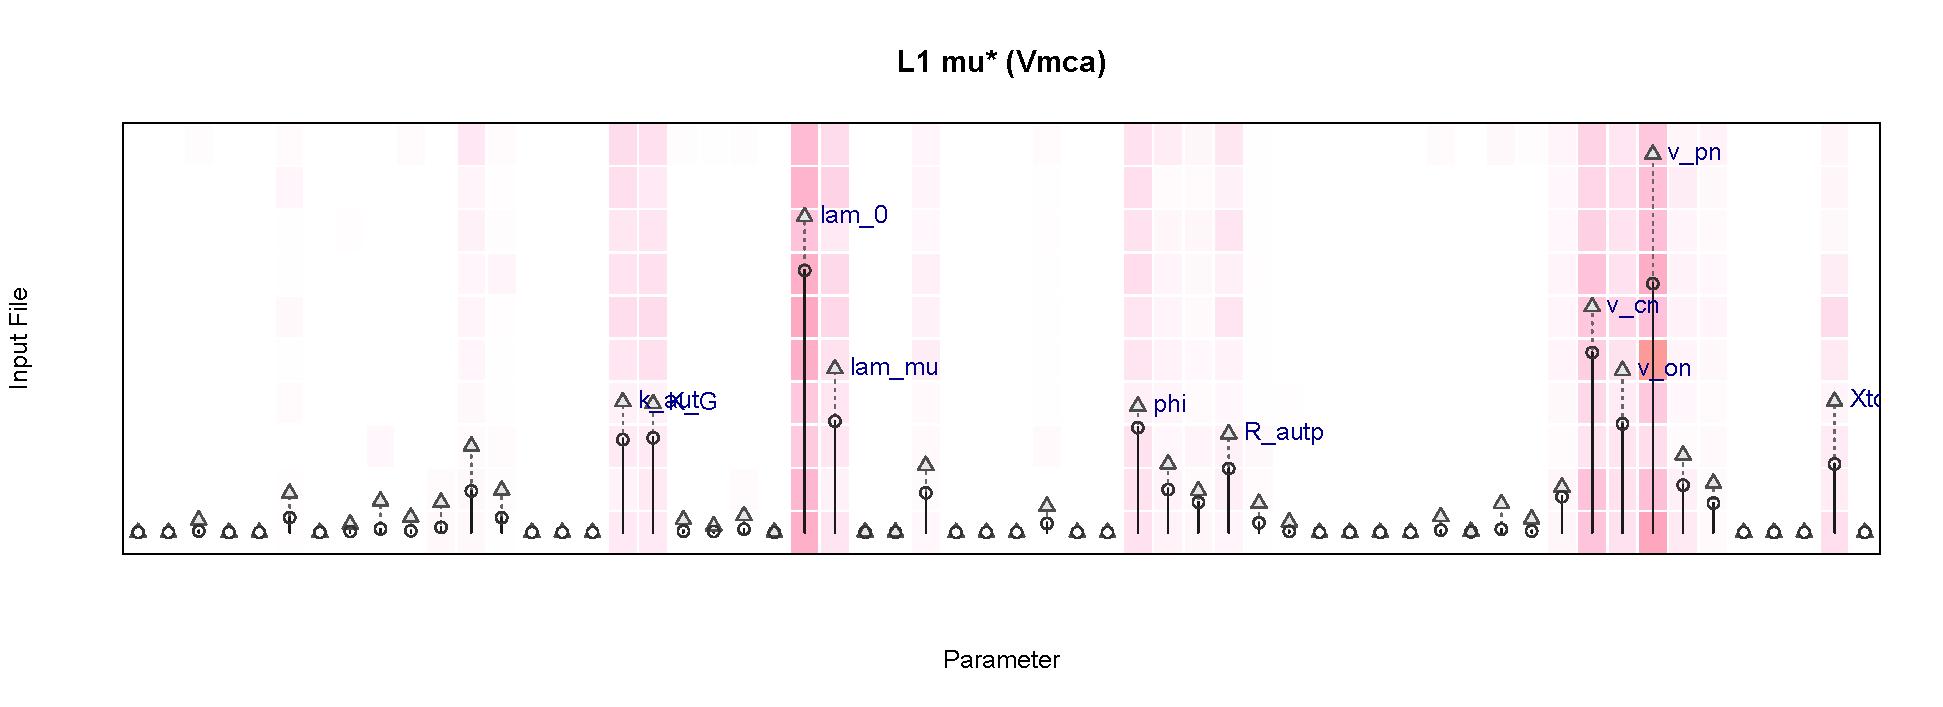
\includegraphics[scale=0.5]{figures/heatmap.pdf}
\caption{A sensitivity `heat map', illustrating differences in parameter sensitivities with different input data.}
\label{fig:batch:heat}
\end{center}
\end{figure}

The script \texttt{aggregate.py} merges \texttt{postproc} output from multiple directories---this can be useful when analysing batches run with different input files. Invoke it like this:
\begin{verbatim}
      python aggregate.py DIR
\end{verbatim}
There are no optional arguments. The required argument \texttt{DIR} specifies the path to a directory that contains a number of subdirectories containing batch results on which \texttt{postproc.py} has already been run. Like \texttt{postproc}, it does not recurse into lower level subdirectories and will skip subdirectories that do not contain useful results.

The script is not at all sophisticated---it assumes that the results are all compatible and makes no attempt to check this or conform them if they aren't. In essence, it just concatenates the contents of the \texttt{elementaries.txt} files from each result set, prefixing an additional column containing the input file as recorded in the \texttt{brief.txt} file. It does not try to enforce uniqueness, so if you run it with more than one directory that was run with the same input then you may get non-unique rows in the output. The merged results are saved to a file called \texttt{aggregate.txt} in the directory specified as \texttt{DIR}.

One of the main reasons for running \texttt{aggregate.py} is to generate data for use in R, to plot the kind of sensitivity `heat map' shown in Figure \ref{fig:batch:heat}. The function that does this is called \texttt{heat\_cross()}, and it can be found in the script \texttt{util.R} in the \texttt{R} directory of the BCMD distribution. The function takes a large number of arguments to configure the plot, but all of them have defaults. In the simplest case, executing \texttt{heat\_cross} in the directory contain the \texttt{aggregate.txt} will load the data and plot the results for one species---the plot in Figure \ref{fig:batch:heat} was generated this way. At some point the full function will be documented here, but in the meantime have a look at the R code, which has relevant comments.

\subsubsection{Optimisation}\label{batch:optim}

The \texttt{optim.py} script attempts to fit the value of one or more model parameters to make the model output resemble a specified target as closely as possible. Optimisation is performed using the OpenOpt Python library (\url{http://openopt.org}), optionally in conjunction with the PSwarm solver \citep[][\url{http://www.norg.uminho.pt/aivaz/pswarm/}]{Vaz:2009wa}. Installing these dependencies is discussed briefly in \S\ref{reqs}, but detailed instructions for all platforms are currently beyond the scope of this document. See the linked sites for more information.

Consider the model as a function $\vv{f}(\vv{x}, t \, | \, \Theta, ...)$, where $\Theta$ denotes the subset of parameters we're interested in. For specified inputs $\vv{x}, t$, let the target output be $\vv{y}$. If $\| \vv{x} - \vv{y} \|_{d}$ denotes distance by some chosen metric $d$, then the `cost' associated with a given parameter combination is
\begin{equation}
 g(\Theta) = \left\| \vv{f}(\vv{x}, t \, | \, \Theta,...) - \vv{y} \right\|_{d}
\end{equation}
and our goal is to determine parameters $\hat{\Theta}$ that minimise $g$. (Note that $g$ is scalar.)

If our models were simple, we wouldn't need BCMD. For most realistic uses, $\vv{g}$ tends to be grossly non-convex and minimisation is a questionable proposition \citep[see][]{Boyd:2004uz}. If you can re-pose your problem in a different, explicit and preferably convex form, such as a linear regression against a prepared body of output data, you are strongly advised to do so. Non-convex global optimisation is, frankly, a mug's game: tedious to set up, computationally expensive, and almost guaranteed to give you the wrong answer to what is probably the wrong question. Alas, sometimes there just aren't any better options available. If you absolutely \textit{must} do this, \texttt{optim} may help; but please be cautious when interpreting the results.

The script is run with Python from the Unix or MSYS command line:
\begin{verbatim}
      python optim.py [options] jobfile datafile
\end{verbatim}
(On Unix platforms the script is executable, and can probably be run directly. However, explicitly including \texttt{python} is more dependable.)

The following command line options are available:
\begin{adjustwidth}{0.8cm}{0.8cm}
\begin{description}
\item[-h, -{}-help] Print a usage message and exit.
\item[-{}-version] Print the program's version number and exit.
\item[-b DIR, -{}-build DIR] Specify the location of the build directory (this is where the model executable is expected to be). The standard BCMD \texttt{build} directory is used by default.
\item[-o DIR, -{}-outdir DIR] Specify a directory for working files and results. The default is a directory \textit{modelname}\texttt{/}\textit{timestamp} inside the specified build directory.
\item[-d, -{}-dryrun] Assemble the data, write the configuration details to \texttt{stdout} and exit without running anything.
\item[-w, -{}-wetrun] Assemble the data, write the configuration details to \texttt{stdout} and do a single test run of the model without subsequent optimisation.
\item[-D, -{}-debug] Run in debug mode, which logs various pieces of information to \texttt{stderr} along the way. If this is specified in addition to \textbf{-{}-wetrun}, the single model invocation does not occur, but the parameters that would be used are printed.
\end{description}
\end{adjustwidth}

The job files for \texttt{optim} are conventionally given the file extension \texttt{.optjob}, although this is not enforced. In addition to the common features described \S\ref{batch:common}, the following keywords are supported:
\begin{adjustwidth}{0.8cm}{0.8cm}
\begin{description}
\item[job\_mode] The kind of OpenOpt job to run. See the OpenOpt documentation for details, such as they are. This should be one of:
	\begin{itemize}
	\item \texttt{GLP}: A global optimisation. This is almost always going to be what you want. Strictly speaking, the whole concept of `global optimisation' is kind of dubious, but anyway.
	\item \texttt{NLP}: A non-linear local optimisation.
	\item \texttt{NSP}: A non-smooth local optimisation. This is much the same as NLP, but with some different default settings.
	\end{itemize}
(Default: \texttt{GLP})
\item[solver] Which optimisation method to use for the problem. Different solvers are supported for the different job modes---seee the OpenOpt documentation for more information. Supported solvers for \texttt{GLP} jobs include the following:
	\begin{itemize}
	\item \texttt{pswarm}: A particle swarm optimisation method. Requires the PSwarm library to be installed, including Python support.
	\item \texttt{galileo}: A genetic algorithm based method. Built into OpenOpt, no external libraries required.
	\item \texttt{de}: A two-array differential evolution algorithm. Built into OpenOpt, no external libraries required.
	\end{itemize}
Other solvers may also work, depending on the nature of the problem and whether you have the relevant external code installed. Pswarm seems to be a good choice for our problems, being somewhat less prone to getting stuck in local minima, but it is often worth trying different solvers and comparing results. (Default: \texttt{galileo})
\item[distance] The distance function to minimise. Value is the actual \textit{name} of the function to call. At present, only functions in the \texttt{distance.py} module are supported, there is no way to specify custom functions elsewhere. One of: \texttt{euclidean}, \texttt{manhattan}, \texttt{loglik}, \texttt{mean}, \texttt{cosine} or \texttt{angular}; see \S\ref{batch:common} for definitions. (Default: \texttt{euclidean})
\item[max\_iter] The maximum number of optimisation iterations to run---fewer will be used if convergence is achieved sooner. This is primarily intended for \texttt{pswarm}, although other solvers may also support it. Iterations in this case are cycles of polling and searching, not model executions. (Default: 1000)
\item[steady] Length of equilibration period at start of each model run (i.e., after setting parameters but before commencing input sequence), in model time units. Set to 0 for no equilibration. (Default: 1000)
\item[timestep] If times are not explicitly provided in the data file, you can optionally choose to specify a default interval and let \texttt{optim} assign the times. In this case, the simulation will start at time 0 and proceed with uniform steps of the specified duration. (No default: if not specified, times must be in the data file.)
\item[weight$^{\dagger}$] A weighting to apply to the distance metric for an output variable. If you are jointly optimising multiple simulated outputs (i.e., if there is more than one \texttt{var} declared), the total cost function $g$ is a weighted sum of the individual signal distances:
$$
	g(\Theta) =  \sum_{v \in \vv{V}} w_v \left\| \vv{f}_v(\vv{x}, t \, | \, \Theta,...) - \vv{y}_v \right\|_{d}
$$
Here, $\vv{V}$ is the set of output variables, while $\vv{f}_v(\cdot)$ and $\vv{y}_v$ are the simulated and target signals for variable $v$. The \texttt{weight} keyword allows specifying $w_v$. The right hand side should contain the variable name as the first element and the numeric weight second:
\begin{verbatim}
      weight: CBF, 0.5
\end{verbatim}
(Default: 1)
\item[post$^{\dagger}$] Specifies some post-processing to apply to a model output variable before calculating the distance. It is sometimes useful to optimise to outputs that have been processed in some way that is difficult to do within the model itself---for example, where you apply some scaling or offset that is derived from the signal. The right hand side gives the name of the variable to which the processing should be applied, followed by a keyword indicating what to do, which may have additional parameters. At present, the following transformations are supported:
	\begin{itemize}
	\item \texttt{zero}: Subtract the initial value from the signal.
	\item \texttt{centre}: Subtract the mean of the signal.
	\item \texttt{norm}: Subtract the mean of the signal and divide by the standard deviation.
	\item \texttt{offset}: Add a specified value to all signal points.
	\item \texttt{scale}: Multiply all signal points by a specified value.
	\end{itemize}
You can specify more than one \texttt{post} for each variable, in which case they are applied in the order they appear in the job file, e.g.:
\begin{verbatim}
      # offset to start from zero
      post: CCO, zero
      # convert units from uM to mM
      post: CCO, scale, 1e-3
\end{verbatim}
(Default: none)
\end{description}
\end{adjustwidth}
As noted by the $\dagger$ symbol, \texttt{weight} and \texttt{post} are multivalued---you may need to specify them for several variables, and indeed you may also specify more than one post processing action for a single variable. All other \texttt{optim}-specific keywords are treated as single-valued: the first occurrence in the file is used, subsequent instances are ignored.

Parameters to be optimised should be given a \texttt{uniform} distribution---the bounds of this are used as box constraints on the parameter value.
Input perturbation is not supported---a distribution can be provided for each \texttt{input} specification, but it will be ignored.

At present, result reporting is extremely basic. The solver may emit various messages as it progresses. Once the job completes, \texttt{optim} prints a short summary to \texttt{stdout}, reporting success or failure and the final values of the optimised parameters. More extensive reporting may be added in future.

%\subsubsection{Approximate Bayesian Computation}\label{batch:abc}
%
%Approximate Bayesian Computation (ABC) attempts to estimate parameter posterior distributions when the likelihood function is unknown or intractable, by using sampling from model simulations as an estimator of the likelihood \citep{Toni:2009ch}. This \textit{should} be useful as a way of providing some quantification on the uncertainties in our estimates, although we have yet to achieve substantive results with it.
%
%The implementation here is based on a drastically cut down version the ABC-SysBio library by \citet{Liepe:2010eg} (\url{http://www.theosysbio.bio.ic.ac.uk/resources/abc-sysbio/}). The original code can generate model implementations based on SBML descriptions, handles job control via a prescribed XML interface, and generates several kinds of plots of the results. This functionality is fine in its own context, but not well-suited for use with BCMD models, so it has all been stripped out. The tattered remnants are included in the \texttt{abcsbh} directory.

\subsection{Direct invocation}\label{direct}

\subsubsection{Compiling}\label{compile}

The BCMD compiler is run with Python from the Unix or MSYS command line:
\begin{verbatim}
      python bparser/bcmd.py [options] model [model ...]
\end{verbatim}
(On Unix platforms the script is executable, and can probably be run directly. However, explicitly including \texttt{python} is more dependable.)

The following command line options are available:
\begin{adjustwidth}{0.8cm}{0.8cm}
\begin{description}
\item[-h, -{}-help] Print a usage message and exit.
\item[-{}-version] Print the program's version number and exit.
\item[-i PATH] Append PATH to default model search path.
\item[-I PATH] Replace the default model search path with PATH.
\item[-n NAME, -{}-name NAME] Specify the name of the model. By default the first model file name is used, with no extension.
\item[-o FILE] Specify output file name. (This is currently unused as the script does not invoke the C compiler itself.)
\item[-d DIR] Specify the directory into which generated files will be placed (default: .)
\item[-u, -{}-unused] Do not calculate apparently-unused intermediate variables. This may be somewhat more efficient, but means that these values cannot be output at runtime.
\item[-g, -{}-debug] Include debug outputs in generated model code. This can be useful for debugging a model, but will make it run more slowly.
\item[-t {[}FILE{]}, -{}-tree {[}FILE{]}] Write the parse tree to a text file. FILE is optional; if not specified, the default is \textit{modelname}\texttt{.tree}
\item[-p {[}FILE{]}, -{}-processed {[}FILE{]}] Write the whole compilation data structure to a text file. FILE is optional; if not specified, the default is \textit{modelname}\texttt{.bcmpl}
\item[-G {[}FILE{]}, -{}-graph {[}FILE{]}] Write the model structure to a GraphViz script. FILE is optional; if not specified, the default is \textit{modelname}\texttt{.gv}
\item[-U, -{}-graphxunused] Exclude apparently-unused variables and parameters from the exported graph.
\item[-N, -{}-graphxinit] Exclude initialisation-only variables and parameters from the exported graph.
\item[-C, -{}-graphxclust] Exclude cluster subgraphs from the exported graph.
\item[-S, -{}-graphself] Include direct circular dependencies (ie, graph edges that loop back to the same node) in the exported graph.
\item[-v LEVEL, -{}-verbose LEVEL] Set the level of detail logged to stderr during compilation (0--7, default: 3)
\item[-Y, -{}-yacc] Run a dummy parse to rebuild the parse tables.
\end{description}
\end{adjustwidth}

The compiler looks for model definition files in the directories specified in the model search path. By default it looks in the current directory and, if present, in a subdirectory called \texttt{models}. It first looks for the specified name exactly as supplied, then tries with the \texttt{.modeldef} extension appended (so it is not necessary to include that). The same search order applies to files imported inside the model definition with the \texttt{@import} directive.

If you are invoking BCMD via the default Makefile targets, the logging output is redirected to \texttt{build/}\textit{modelname}\texttt{.log}---this is the first place to look if you encounter a problem compiling. If there is an error in your model definition it will usually at least tell you what line it's on and what parse token caused the error. This doesn't necessarily diagnose the problem but it should help at least a little bit.

The generated C code file must be compiled and linked with the RADAU5 library. The \texttt{\%.model} target in the Makefile takes care of this (and does not assume you are using the default \texttt{build} directory). If you prefer to compile without using this target, check the Makefile for the requisite compiler options, which should have been identified by the \texttt{configure} script.

See \S\ref{info} below for more information on the graph generation options.

\subsubsection{Running}\label{runtime}

The compiled model program can be run from the command line. The following options are available:

\begin{adjustwidth}{0.8cm}{0.8cm}
\begin{description}
\item[-h, -{}-help] Print a usage message and exit.
\item[-v, -{}-version] Print the model version information and exit.
\item[-m, -{}-model] Print the model name and exit.
\item[-s, -{}-symbols] Print a list of the symbols (i.e., the variable and parameter names) used in the model, together with their initial values. The latter are given after the model has initialised, but before anything specified in the input file. After printing, the program exits.
\item[-i FILE, -{}-input FILE] Specify an input file with which to run the model. If no input is specified, the model is run for a single time step of 1000 time units (typically seconds), with all parameters initialised to their default values.
\item[-I, -{}-stdin] Take input from \texttt{stdin} rather than a file. Note that if both this option and \texttt{-{}-input} are provided, whichever comes last will take precedence.
\item[-o FILE, -{}-output FILE] Specify an output file for coarse results (see below). If this is not specified, the results are printed to \texttt{stdout}.
\item[-d FILE, -{}-detail FILE] Specify an output file for detailed results (see below). If this is not specified, detailed results are not printed.
\item[-N, -{}-NaN] Initialise all working data (variables and parameters) with NaN values instead of 0. This may be useful in diagnosing problems with the model. (May not work on all platforms.)
\end{description}
\end{adjustwidth}

As described in \S\ref{input}, a model run is controlled by an input data file, which specifies time steps and parameter changes. For each time step in the input, the RADAU5 solver is invoked. During this invocation the model equation system may be evaluated at many intermediate time points. The calculated values at these time points are reported in the \textit{detailed} output. The values at the end of the time step, after RADAU5 returns, are reported in the \textit{coarse} output. The two sets of output are sent to different destinations and can be configured by the input file to report different data.

At present, results data are written in tab-delimited text format, usually with a header row (though that can be set by the input file). No internal plotting facilities are provided, nor are they likely to be---that sort of thing is much better handled in R or Matlab. (For very simple cases, the results can be plotted with \hyperref[bgui]{BGUI}.)

If you are running the model via the default Makefile targets, the coarse outputs are saved to the file \texttt{build/}\textit{modelname}\texttt{.out} and the detailed ones to \texttt{build/}\textit{modelname}\texttt{.detail}. In addition, the standard output and error streams are redirected to the files \texttt{build/}\textit{modelname}\texttt{.stdout} and \texttt{build/}\textit{model\-name}\texttt{.stderr}. If the model was built in debug mode (the Makefile default), the latter file may be very large.

\begin{figure}[tbph]
\begin{center}
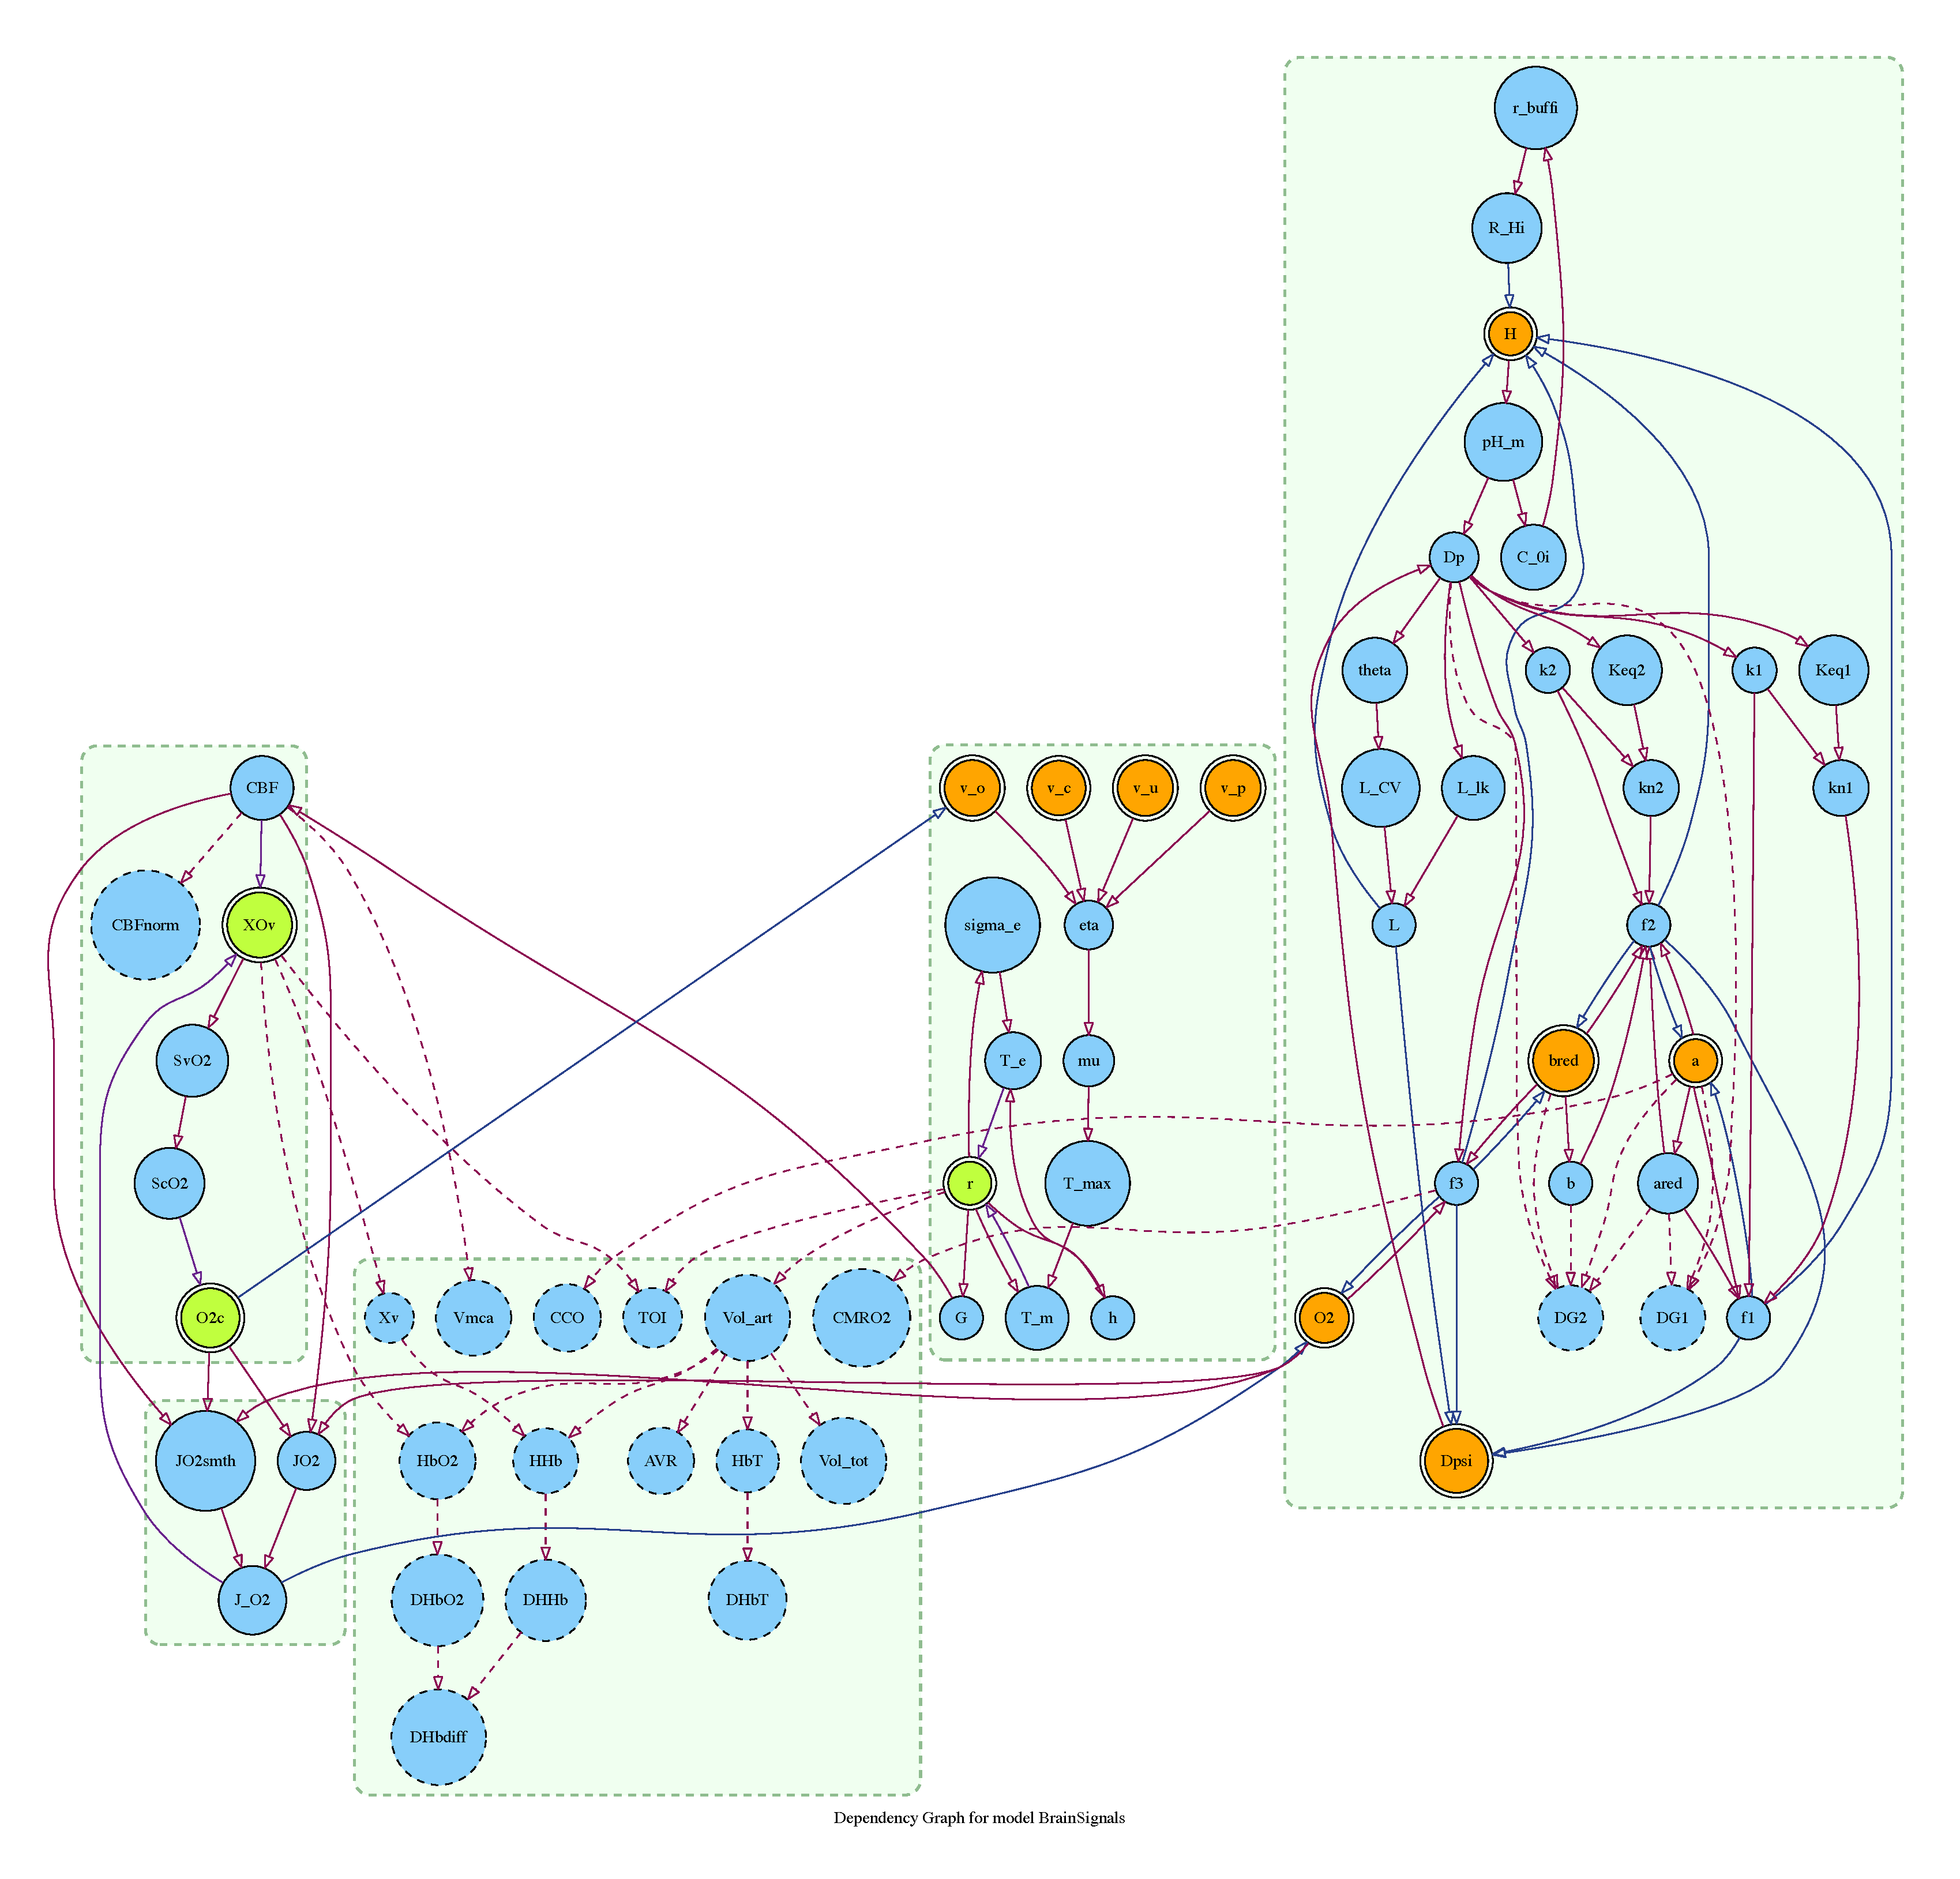
\includegraphics[scale=0.25]{figures/graph.pdf}
\caption{Dependency graph of the BrainSignals model, with parameters omitted. Variables are clustered into subgraphs according to tags in the model.}
\label{fig:graph}
\end{center}
\end{figure}

\subsubsection{Info}\label{info}

The compiler tools include a module for extracting some useful information about a model after it has been compiled, generating model documentation and generating graphs of its structure like the one in Figure \ref{fig:graph}. This is invoked automatically to print some summary information when compiling, and is also used by BGUI, so it is usually not necessary to call it directly. Nevertheless, it is sometimes useful to do so, running it from the command line like this:
\begin{verbatim}
      python bparser/info.py [options] file
\end{verbatim}
The \texttt{file} argument should be the name of the \texttt{.bcmpl} parser information file generated when a model was compiled (so compilation must have included the \texttt{-p} option). Both BGUI and the Makefile place these files in the \texttt{build} directory.

The following options are available:

\begin{adjustwidth}{0.8cm}{0.8cm}
\begin{description}
\item[-h, -{}-help] Print a usage message and exit.
\item[-d DIR] Specify output directory (default: .)
\item[-t {[}FILE{]}, -{}-text {[}FILE{]}] Specify output of model documentation in plain text format. FILE is optional, if omitted the output file is called \textit{modelname}\texttt{.txt}
\item[-l {[}FILE{]}, -{}-latex {[}FILE{]}] Specify output of model documentation in \LaTeX{} format. FILE is optional, if omitted the output file is called \textit{modelname}\texttt{.tex}
\item[-H {[}FILE{]}, -{}-html {[}FILE{]}] Specify output of model documentation in HTML format. FILE is optional, if omitted the output file is called \textit{modelname}\texttt{.html}
\item[-m {[}FILE{]}, -{}-modeldef {[}FILE{]}] Specify output of a consolidated model definition. FILE is optional, if omitted the output file is called \textit{modelname}\texttt{.modeldef}
\item[-S {[}FILE{]}, -{}-sbml {[}FILE{]}] Specify export of model to SBML format. FILE is optional, if omitted the output file is called \textit{modelname}\texttt{.xml}
\item[-a] Generate all major graph variants, using their default names.
\item[-n NAME, -{}-name NAME] Specify a model name instead of deriving it from the file.
\item[-U {[}FILE{]}, -{}-graphxunused {[}FILE{]}] Produce graph with unused elements omitted. FILE is optional, if omitted the output file is called \textit{modelname}\texttt{\_no\_unused.gv}
\item[-N {[}FILE{]}, -{}-graphxinit {[}FILE{]}] Generate graph with initialisation dependencies omitted. FILE is optional, if omitted the output file is called \textit{modelname}\texttt{\_no\_init.gv}
\item[-P {[}FILE{]}, -{}-graphxparam {[}FILE{]}] Generate graph with parameters omitted. FILE is optional, if omitted the output file is called \textit{modelname}\texttt{\_no\_params.gv}
\item[-X {[}FILE{]}, -{}-graphcore {[}FILE{]}] Generate graph excluding both initialisation and unused elements. FILE is optional, if omitted the output file is called \textit{modelname}\texttt{\_core\_only.gv}
\item[-C {[}FILE{]}, -{}-graphxclust {[}FILE{]}] Output graph without clustering. FILE is optional, if omitted the output file is called \textit{modelname}\texttt{\_no\_clusters.gv}
\item[-F {[}FILE{]}, -{}-graphfull {[}FILE{]}] Output graph with everything included. FILE is optional, if omitted the output file is called \textit{modelname}\texttt{.gv}
\item[-R, -{}-graphself] Include direct circular dependencies in graphs.
\item[-s, -{}-summary] Print summary information to \texttt{stdout}.
\item[-x, -{}-nograph] Suppress all graph output.
\item[-v LEVEL, -{}-verbose LEVEL] Set output verbosity (0--7, default: 5)
\end{description}
\end{adjustwidth}

At present there are no formatting options for the documentation files produced when invoking this module from the command-line. The default formatting is always used. If you wish to apply different \LaTeX{} formatting, you must access these via the BGUI Info panel (\S\ref{bgui:info}).

Most of the graphing options should be reasonably self-explanatory. Initialisation dependencies are those that only occur before the solver is first called, typically to set initial values and calculate derived parameters. Unused variables are intermediates that do not feed back to the behaviour of the model variables, often used for output processes. Parameters are values that have no dependence on model variables. Clusters are boxes that group together symbols sharing the same primary tag (\S\ref{model:tags})---if tags have not been assigned, then omitting clusters has no effect.

It is possible to generate more than one graph in a single run, and indeed doing so is necessary to obtain some variations: to avoid having options for every possible combination, there is some interaction between types. For example, if producing both parameterless and clusterless versions, the latter will also exclude parameters.

The graph generation features produce \texttt{.gv} files containing a specification of the graph in the GraphViz DOT language. To convert these to actual graphics, you need to have the \href{http://www.graphviz.org}{GraphViz} tools installed. These provide a range of different transformation options, for which you'll need to examine the GraphViz documentation. However, the following command provides a reasonable starting point for most purposes:
\begin{verbatim}
      dot -Tpdf -o model.pdf  model.gv
\end{verbatim}
This generates a PDF version of the graph described in \texttt{model.gv} (substitute the actual name as appropriate).

For the moment, no control is provided over the appearance of the generated graphs---the styling for different element types is as always as shown in Figure \ref{fig:graph}. This is likely to change in future.

\section{Model definition}\label{models}

Models are defined in one or more plain text files. Definitions can contain any of the following elements:

\begin{itemize}
\item differential equations
\item algebraic equations
\item chemical reactions
\item constraints
\item arbitrary intermediate variables and parameters
\end{itemize}

In addition, files can contain comments (which begin with a \texttt{\#} symbol) and some other directives for doing things like importing other files (which begin with an \texttt{@} symbol). The elements can be defined in any order and none are compulsory---although obviously a definition that doesn't give rise to a meaningful equation system will not run sensibly (and in some cases might cause compilation to fail, though we hope to catch most such cases eventually).

\subsection{Comments and whitespace}
Comments allow the inclusion of arbitrary text in a model definition file, to provide human-readable notes and documentation\footnote{The BCMD modelling language is designed with a philosophy almost diametrically-opposed to that of some other languages, such as SBML. We assume that you know what you want to do, and attempt to let you do it as directly and concisely as possible. Therefore, much of the model structure is implicit. You are not required to specify what everything is or how you expect it to behave, and there is no support for automatic checking or conversion of things like units. Consequently, while it is much easier to do things \textit{at all} in a BCMD model than in a bureaucratic environment like SBML or CellML, it is also quite easy to get things horribly wrong. We recommend structuring your model code as cleanly and intuitively as you can, making liberal use of comments and spacing to aid readability.}. They begin with a hash character \texttt{\#}, may start anywhere on a line and then continue to the end of that line. Comments are essentially ignored and in general do not contribute to the model definition (though there is at least one minor exception to this, described below).

Most other model elements must start at the beginning of the line. Conceptually, they occupy a single line in the file, but continuation across multiple lines is allowed using indentation: any line that starts with whitespace characters is considered to be a continuation of the previous line (with any tail comments stripped off). That is, something like this:
\begin{verbatim}
      x = (a                # some comment about a
           + b)             # some comment about b
\end{verbatim}
is equivalent to:
\begin{verbatim}
      x = (a + b)
\end{verbatim}
The amount of indentation is unimportant, so different lines can be indented differently. This can be useful for keeping track of complex nested parentheses, for example.

Otherwise, whitespace is ignored.

\subsubsection{Documentation comments}\label{model:doc:comments}
Comments beginning with a double hash \texttt{\#\#} are recognised as a distinct type. Like normal comments, they have no effect on the model itself (with one exception, noted below), but they provide additional information which is used when automatically generating model documentation (\S\ref{bgui:info} and \S\ref{info}).

Several special cases of documentation comment, described below, are specified by their first non-comment character. Otherwise, doc comments simply contain text that will be included \textit{almost} verbatim in the generated documentation.

The exact treatment varies with the documentation generator. The HTML generator escapes HTML special characters in the doc comments, so you can use the $<$, $>$ and \& characters freely, but you cannot embed links or HTML styling. On the other hand, the \LaTeX{} generator does not escape special characters, so it is possible to embed \LaTeX{} commands, but also quite easy to accidentally break your document with a misplaced underscore or ampersand. Plain alphanumeric text should produce sensible output for all generators, but of course that may not suit your purposes.

An empty doc comment denotes a paragraph break.

\subsubsection*{Attachment comments}
All doc comments are attached to either a model symbol---a parameter or variable---or to the model as a whole. (At present it is not possible to attach comments to an equation or chemical reaction.) Comments are usually expected to be attached to whatever is defined immediately after them in the file:
\begin{verbatim}
      ## Some lines of information about the variable x,
      ## perhaps describing its relationship to a and b.
      ##
      ## A second paragraph of information about x.
      x = a + b
\end{verbatim}
However, it is sometimes inconvenient to position them in this way, and we may also want to attach the current comments to a number of separate entities---this is often the case for \textit{tags} (see below) for example. To allow this, doc comments that begin (after the hash characters themselves and any whitespace) with an at character \texttt{@} are taken as specifying one or more symbols to which the most recent comment(s) should be attached. E.g.:
\begin{verbatim}
      ## This parameter has no effect on simulation behaviour,
      ## it is purely for output purposes.
      ## @ hue saturation brightness
\end{verbatim}
Here, the same comment would be attached (separately) to each of the three symbols listed.

An \texttt{@} comment with no targets tells the compiler to attach the comments to the model itself rather than to any specific symbol within it.

Note that you can attach comments to symbols that you have not yet defined, but doing so \textit{creates} the symbol---that is, if you attach a comment to a symbol, then that symbol exists in the model, even if you never subsequently define it. It won't actually \textit{do} anything in that case, and will have no material effect on the model. However, we often use counts of variables and parameters as a rough metric of model size, and spurious unused symbols could be misleading in that regard.

\subsubsection*{Tags}\label{model:tags}
A doc comment beginning (after the hash characters and any whitespace) with a plus sign \texttt{+} is considered to define one or more keywords or \textit{tags} to associate with a model symbol. These might be used, for example, for classifying symbols according to the processes in which they participate. Tags are whitespace separated, and should follow the rules for variable identifiers (\S\ref{vars}).
\begin{verbatim}
      ## + horizontal mysterious adults_only marks_the_spot
      x = a + b
\end{verbatim}
Symbols can have any number of tags attached to them, but the \textit{first} one declared for each symbol is considered its `primary' tag. The graph generator makes special use of this tag: if clustering is enabled (as it is by default), all symbols with the same primary tag are clustered together into the same subgraph. (See Figure \ref{fig:graph} for an example.)

\subsubsection*{Units}\label{model:units}
A doc comment beginning (after the hash characters and any whitespace) with a tilde character \texttt{\~} specifies what units the variable or parameter is measured in. This is purely informational, and is not interpreted or used in any way by the model. \LaTeX{} markup is allowed in the units, but will obviously look odd when generating HTML or plain text documentation.
\begin{verbatim}
      ## X is the speed of an Arcturan Mega-Donkey's soul
      ## ~ furlongs/fortnight
      x = a + b
\end{verbatim}

\begin{table}[tbp]
\begin{center}
\begin{tabular}{| c | c |}
\hline
Name					& Default Appearance \\
\hline
\texttt{tigers}				& $tigers$ \\
\texttt{\_\_tigers\_\_}			& $tigers$ \\
\texttt{tiger\_cubs}			& $tiger_{cubs}$ \\
\texttt{\_X\_y\_z\_abc\_d\_}	& $X_{y,z,abc,d}$ \\
\hline
\end{tabular}
\end{center}
\caption{Examples of the default symbol name rendering by the \LaTeX{} documentation generator.}
\label{tab:latex:default}
\end{table}

\subsubsection*{\LaTeX}\label{model:latex}
A doc comment beginning (yes, you guessed it, after the hash characters and any whitespace) with a dollar sign \texttt{\$} specifies a \LaTeX{} math mode fragment to be used to represent a symbol in generated \LaTeX{} documentation. The fragment substitutes for the plain text symbol used in the model definition itself. For example, you could do something like this:
\begin{verbatim}
      ## A small amount. Less than this we just don't care.
      ## $ \varepsilon
      ## @ epsilon
\end{verbatim}
Within generated \LaTeX{} documentation, the model symbol \texttt{epsilon} would then be rendered as $\varepsilon$ rather than $epsilon$. It is not necessary to provide a closing dollar sign, but you may do so if you wish.

If you \textit{don't} specify a \LaTeX{} fragment explicitly, the \LaTeX{} documentation generator gives special treatment to symbol names containing underscores. First, any underscores at the beginning and end of the symbol are removed. Anything before the first internal underscore is treated as the main symbol, and everything after is placed as a subscript. If there are multiple underscore-separated parts to the subscript, these become comma-separated in the subscript. Some examples are shown in Table \ref{tab:latex:default}. This rendering may be sufficient to your needs, in which case it is fine to rely on it. Note however, that there is no attempt to ensure uniqueness---if you have symbols in your model that differ only by leading or trailing underscores, they will be rendered identically in the documentation.

\subsection{Compiler directives}
Compiler directives begin with an at character \texttt{@}. At present there are six of these, described below.

\subsubsection{@import}
This directive tells the compiler to include other files into the current model. The \texttt{@import} keyword is followed by one or more model names, delimited by whitespace. E.g.:
\begin{verbatim}
      @import submodel shared_params
\end{verbatim}
Note that at present the names must follow the rules for variable identifiers (\S\ref{vars}), and thus cannot include a filename extension. (This will probably change in future.) The compiler searches for these files in the same way as for source files specified on the command line (\S\ref{compile}).

\subsubsection{@version}
This directive specifies a version number or string to be associated with the model. This is optional, but can be useful for keeping track of changes. If the version is a number, or if it conforms to the variable identifier rules (\S\ref{vars}), then it can follow the directive without quoting. Otherwise surround it in double quotes. E.g.:
\begin{verbatim}
      @version 1.2
      @version "1.2 (simplified)"
\end{verbatim}
The version string for a compiled model can be queried by running the model with the \texttt{--version} option (\S\ref{runtime}).

\subsubsection{@independent}
This directive specifies the name of the independent variable used in the equation system. By default, this is \texttt{t}. Note that most of our models do not include an explicit dependence on the independent variable and don't need to refer to it by name, but it may be useful to do so for cosmetic or readability reasons. E.g.:
\begin{verbatim}
      @independent x
\end{verbatim}

\subsubsection{@output}\label{at:output}
This directive specifies which variables should be output when no other output specification has been made in the input file, or when the input file specifies \texttt{*} (see \S\ref{input}). By default, all solver variables are included in this output.

The \texttt{@output} keyword is followed by one or more variable or parameter names, delimited by whitespace. Multiple such directives can be included in a file, and all variables specified in all of them will be output. E.g.:
\begin{verbatim}
      @output x y z
      @output v w x
\end{verbatim}
Note that the independent variable (by default \texttt{t}, but see the \texttt{@independent} directive above), is always included as the first column of the default output. Each symbol is only added to the output once, so in the above example the second \texttt{x} will be ignored. Symbols that are not actually declared in the model are also ignored.

\subsubsection{@input}\label{at:input}
This directive specifies which variables are intended to be used as model inputs. Note that this exists largely for information purposes and is not binding---you can still set any parameters you want in the input file.

The \texttt{@input} keyword is followed by one or more variable or parameter names, delimited by whitespace. Multiple such directives can be included in a file, and all variables specified in all of them will be marked as inputs. E.g.:
\begin{verbatim}
      @input x y z
      @input v w x
\end{verbatim}
Any symbols not actually declared in the model are ignored.

It is expected that this will be used for additional model checking in the future. However, at present it only really affects the summary information generated by the compiler, and the order in which symbols are displayed in some parts of the BGUI interface.

\subsubsection{@extern}\label{at:extern}
This directive identifies variables that are \textit{referenced} in the current model, but which are expected to be \textit{defined} elsewhere. This is really only relevant when models are broken down into several different files that may be combined in different variations. Once again, this is purely informational.

The \texttt{@extern} keyword is followed by one or more variable or parameter names, delimited by whitespace. Multiple such directives can be included in a file, and all variables specified in all of them will be marked as potentially external. E.g.:
\begin{verbatim}
      @extern x y z
      @extern v w x
\end{verbatim}
When the model is compiled, any symbols not actually referenced in the model are ignored. Symbols that are defined in the model (i.e., assigned a value or expression, rather than merely referenced) are also ignored. Whatever remains is treated as an ordinary parameter, but is reported as external in generated graphs and documentation.

The idea here is that when you break a model up into separate parts, you mark important connecting elements as external. If the submodels are compiled together, the external dependencies are satisfied and the symbols become just an ordinary part of the joint model. On the other hand, if you compile the submodels singly or in incomplete combinations, the unsatisfied \texttt{@extern} dependencies will be reported.

\subsection{Embedded C}\label{embeds}
Unlike BRAINCIRC, the expressions in a BCMD model definition are not literal C code and do not get directly included in the generated C file. However, it is possible to add C code fragments by surrounding them with the special delimiters \texttt{[**} and \texttt{**]}. Everything between these will be copied verbatim into the generated file.

Since the resulting code is unchecked, this should be done sparingly, but it can be useful for defining functions that are not included in the standard C libraries. E.g.:
\begin{verbatim}
      [**
      /* Simple Heaviside step function. */
      double heavi(double s)
      {
          return (s < 0.0) ? 0.0 : 1.0;
      }
      **]
\end{verbatim}
Note that arbitrary variable names or \texttt{\#define} constants created in embedded C code \textit{cannot} be directly accessed from within BCMD expressions. Functions to be invoked within BCMD expressions should have a return type of \texttt{double}, which should also be the type for any parameters taken.

\subsection{Expressions}

\subsubsection{Variable identifiers}\label{vars}
Variable identifiers are placeholders for any numerical quantity in the model, including chemical species, parameters and compartments. Identifiers are made up of alphanumeric characters and underscores, and must not start with a number. There is no explicit length limit. Thus, \texttt{x}, \texttt{CO2} and \texttt{unreasonably\_long\_parameter\_name} are all valid identifiers, but \texttt{5HT} and \texttt{O2\%} are not.

Variables do not need to be declared before use. They are automatically created the first time they are used, and their type is determined from context. If they appear in several different equations with conflicting requirements, an error will be reported.

A variable that is used but never given a value in the model definition is automatically initialised with the value \texttt{0}. All variable values may be overridden at runtime.

Note that BCMD variable names \textit{do not} map to C variable names. You cannot access them directly from embedded C code.

\subsubsection{Numbers}\label{nums}
All numbers in BCMD are ultimately handled in double-precision floating point form. It is not necessary to include a decimal point for type distinction purposes. Numbers can be specified in `engineering' notation if desired. The following are all valid numbers:
\begin{verbatim}
      9
      -1.0
      1.2e-5
      2E6
\end{verbatim}

\subsubsection{Mathematical operators}
Arithmetic is performed with the usual operators: \texttt{+}, \texttt{-}, \texttt{*} and \texttt{/}, while \texttt{\^} signifies exponentiation. Addition and subtraction have lower precedence than multiplication and division, exponentiation has higher, and all these operators associate to the left. Precedence can be overridden using parentheses, e.g.:
\begin{verbatim}
      (a + b)/c
\end{verbatim}

\subsubsection{Comparisons and conditionals}
Comparisons between numerical values are made using the following operators \texttt{==}, \texttt{!=}, \texttt{>}, \texttt{>=}, \texttt{<} and \texttt{<=}, which have their conventional interpretation. The result of a comparison is a logical (true or false) value; unlike in C, these cannot be freely mixed with numerical values. They have meaning only in the context of the \textit{conditional operator}, \texttt{?:}, which is equivalent to an \textit{if ... else ...} construct:
\begin{verbatim}
      (a == b) ? c : d
\end{verbatim}
In this example, the whole expression takes the (numerical) value \texttt{c} if the test (\texttt{a==b}) is true, otherwise it takes the value \texttt{d}.

\subsubsection{Function invocation}
A function call is denoted with parentheses in the usual way: \texttt{function(arg1, arg2, ...)}. All functions are assumed to return a numerical value and take numerical arguments. Because of this, you cannot use a function call on its own in the condition term of a conditional operator expression:
\begin{verbatim}
      # this is not allowed
      sometest(a) ? b : c
      
      # but this is
      sometest(a) != 0 ? b : c
\end{verbatim}
All the functions of the C standard maths library (from \texttt{<math.h>}) are included by default.

\subsection{Equations}\label{eqs}
Differential, algebraic and arbitrary temporary variable equations have similar forms. All use the single equals character \texttt{=} to declare the relation. The right hand side in all cases is a mathematical expression, of arbitrary complexity, plus an optional double-quoted label. The left hand side determines the type of the equation.

The following are syntactically valid examples of each of the three types:
\begin{verbatim}
      temp = a + b * c / sqrt(d)          "intermediate"
      diff' = temp * diff                 "differential"
      alg : 0 = 2 * alg - diff            "algebraic"
\end{verbatim}
The quoted labels are effectively cosmetic, included primarily for consistency with BRAINCIRC. They can safely be omitted, and in most cases probably should; use comments instead.

The different forms of the left hand side are explained below.

\subsubsection{Intermediate variables}\label{temps}

Intermediate or temporary variables are the simplest kind of equation. They specify an expression that is used within the model, or that you might want to output when simulating, but without declaring a variable for which the system is to be solved (i.e., a member of the $\vv{y}$ vector in Equation \ref{eq:general}). The right hand side in this case is simply the name (identifier) to be used to refer to the expression:
\begin{verbatim}
      name = expression
\end{verbatim}
See \S\ref{eval} for a discussion of when intermediate variables get evaluated.

\subsubsection{Differential equations}\label{diffs}

A differential equation defines one row of the general matrix equation in Equation \ref{eq:general}. This means that it declares both a variable in the $\vv{y}$ vector, and also a row in the mass matrix $\vv{M}$. The former is done by the first term on the left hand side; the second by that taken together with any further left hand terms. In the simplest (and thankfully most common) case, there is only the one term, and the expression will look like this:
\begin{verbatim}
      name' = expression
\end{verbatim}
(Note the apostrophe character to indicate differentiation.)

More complex cases specify linear relationships between the differential terms, corresponding to off-diagonal elements in $\vv{M}$. They are specified like this:
\begin{verbatim}
      name' + w1 name1' + w2 name2' + ... = expression
\end{verbatim}
i.e., as a weighted sum of differential terms on the left hand side. The weight of the first term is always implicitly 1 and must not be included. The other weights must (for the moment at least) be numeric literals (and can be omitted if 1). For negative terms, use a \texttt{-} operator instead of \texttt{+}. E.g.:
\begin{verbatim}
      u' + 2 v' - w' = u + x / y
\end{verbatim}
All left hand side terms must be differentials, and the secondary ones must each also occur elsewhere in the model as the primary term in a differential equation in their own right (otherwise $\vv{M}$ cannot be constructed).

\subsubsection{Algebraic equations}\label{diffs}

Like differential equations, algebraic equations define a row of the general matrix equation in Equation \ref{eq:general}, but in this case the corresponding row of $\vv{M}$ is set to 0. Thus the natural form of an algebraic relation would be like this:
\begin{verbatim}
      0 = expression
\end{verbatim}
However, it is also necessary for the equation to declare a variable in $\vv{y}$. Since in many cases this will be ambiguous, we do not attempt to have the parser guess the variable from the expression, but instead require it to be specified explicitly on the left hand side, in this form:
\begin{verbatim}
      name : 0 = expression
\end{verbatim}
In some cases it is more intuitive to represent the equation part in the form \texttt{expr1 = expr2} rather than \texttt{0 = expr2 - expr1}, so this is also supported. E.g.:
\begin{verbatim}
      T_v1 : T_v1 = sigma_v1 * h_1
\end{verbatim}

\subsection{Initial values}\label{inits}

Initial values for variables and parameters may be specified by using a Pascal-style operator \texttt{:=} for assignment:
\begin{verbatim}
      name := expression
\end{verbatim}
Apart from the change of symbol, the syntax is identical to that for temporary variables, with arbitrary expressions, function calls etc allowed on the right hand side, as in this example from the Ursino-Lodi model definition:
\begin{verbatim}
     T_m1n := T_max1n*exp(-pow(fabs((r_1n-r_m1)/(r_t1-r_m1)), n_m1))
\end{verbatim}
Initialisation differs from intermediate variable definition in that the expression is \textit{only} evaluated at the beginning of the simulation, \textit{even if it includes dependencies on other parameters or solver variables}. See \S\ref{eval} for a full discussion of this.

\subsection{Constraints}\label{constraints}
Constraints represent simple bounds on the values taken by a variable. There are nominally two forms, \textit{hard} and \textit{soft}, although the latter are not yet properly implemented in the model code.

\subsubsection{Hard constraints}\label{hard}
Hard constraints are declared like this:
\begin{verbatim}
      variable > expression
\end{verbatim}
(the operators \texttt{<}, \texttt{<=} and \texttt{>=} can also be used). Note that this is a declaration of the desired state rather than the test for violation as in BRAINCIRC. I.e., the above statement asserts that \texttt{variable} must always exceed \texttt{expression}. The constraint need not be constant.

The constraint is `hard' in the sense that is enforced: if the variable goes across the barrier value, it is set back to it. (It should be noted that this means the strict constraints \texttt{<} and \texttt{>} are not properly observed, since we can't meaningfully set the variable value to an infinitesimal offset from the boundary.)

By far the most common constraint is non-negativity (\texttt{variable >= 0}). This is automatically imposed for all species in chemical equations, so does not need to explicitly declared in such cases.

\subsubsection{Soft constraints}\label{soft}
Soft constraints are declared like this:
\begin{verbatim}
      ~ variable > expression
\end{verbatim}
i.e., the same as hard constraints but prefixed with a tilde character \texttt{\~}.

Soft constraints are not enforced, and at present there is no way of outputting them, so they basically do nothing. The intention is that violations will be noted and it will be possible to output them and potentially act accordingly (e.g., by prematurely halting a simulation run). This is not currently at the top of the `to do' list.

\subsection{Chemical reactions}\label{chem}
Reactions are declared in a sort of caricatured chemical equation form. Reactant and product concentrations are essentially just normal variables, but with some additional notation to distinguish the context. Each reaction participant is enclosed in square brackets, like this:
\begin{verbatim}
      [chemical]
\end{verbatim}
Optionally, the chemical may be associated with a particular compartment:
\begin{verbatim}
      [chemical, compartment]
\end{verbatim}
Both elements (if present) must be single identifiers. If a compartment is present, it is assumed to refer to a variable or parameter that holds the compartment \textit{volume}, so that the actual chemical concentration in the compartment is $chemical \div compartment$. (When no compartment is given, that is equivalent to one of unit volume.)

It is important to note that a chemical present in two different compartments is actually considered as two different chemicals. If there is a flux between the compartments, this should be specified as a reaction. If you need to refer to the species quantity in a mathematical expression other than a chemical reaction, the implicitly-created species variable name consists of the species name and the compartment name joined by an underscore. Moreover, the value of this variable is an \textit{absolute quantity} rather than a concentration---for the latter you must divide by the volume. E.g.:
\begin{verbatim}
      # entry of O2 into mitochondrial compartment
      -> [O2, mit] {J_O2}
      
      # intermediate variable for the mitochondrial O2 concentration
      mitO2 = O2_mit / mit
\end{verbatim}
(The way this is structured is frankly confusing, and may be made more intuitive in future.)

Reactions are specified with the right arrow operator \texttt{->} for a one-way reaction, or the double arrow operator \texttt{<->} for two-way (the latter is essentially just a shorthand for two opposing one-way reactions). The terms on each side consist of some number of of participants, each with an optional weight expression, separated by \texttt{+} signs. Finally, there are one (for one-way reactions) or two (for two-way) reaction rate expressions in curly braces. E.g.:
\begin{verbatim}
      4 [a, comp1]  <-> 2 [b] + X [c, comp2] {k1} {MA:k2}
\end{verbatim}
The weights can be any mathematical expression, although if it's very complex it's probably clearer to make it an intermediate variable. In the one-way form, one or other side can be empty, denoting the supply (left hand empty) or removal (right hand empty) of reactants. E.g.:
\begin{verbatim}
      # a supply reaction from the BrainSignals model
      -> [O2, Vol_mit] {J_O2}
\end{verbatim}
Each reaction rate may be specified explicitly in full, using any mathematical expression, or it may be prefixed with a label (followed by a colon) indicating a standard form. Currently, two such forms are supported: \textit{mass action}, indicated by the prefix \texttt{MA}, and \textit{Michaelis-Menten}, with the prefix \texttt{MM}. (If some other unrecognised prefix is used, the rate term is treated as explicit.)

Note that the in the case of two-way reactions, the rate term in each direction is completely distinct. They are not required to be of the same type---if you wish them to be, that type must be specified in both terms.

\subsubsection{Mass Action kinetics}\label{mak}

For mass action kinetics, the reaction rate is dependent on the concentrations of the reactants. The dependence is assumed linear by default, but you can optionally specify a power law expression for each reactant.\footnote{This differs from BRAINCIRC, which would automatically raise each concentration to the power of the stoichiometry. That is a valid approximation in the case of elementary reactions, but does not apply more generally. Since it would be difficult to distinguish between cases automatically---and since such rate laws are always empirical anyway---BCMD requires the power to be specified appropriately.}

At least one rate expression \textit{must} be supplied, to indicate the proportionality, while additional expressions may be included for the powers. The latter are applied to the the reactant terms in left-to-right order; chemicals for which no power is supplied are assumed to contribute linearly.

E.g., the following reaction with a mass action rate specified as:
\begin{verbatim}
     2 [A] + [B] -> [C] {MA : k, 2}
\end{verbatim}
is equivalent to this one where the rate is specified explicitly:
\begin{verbatim}
     2 [A] + [B] -> [C] {k * A^2 * B}
\end{verbatim}

\subsubsection{Michaelis-Menten kinetics}\label{mmk}

For Michaelis-Menten kinetics, the reaction is assumed to occur via the formation of an intermediate complex with an enzyme, present at low concentration. The enzyme is not consumed and is not included explicitly in the chemical equation, but instead enters via a limiting rate value $V_{max}$ and complex breakdown/formation ratios for each substrate, $K_{m1}$, $K_{m2}$, ... These values must be supplied in the rate term definition, starting with $V_{max}$ and then the $K_{m}$ expressions in the same order as the reactants appear on the relevant side of the reaction:
\begin{verbatim}
      n1 [S1] + n2 [S2] -> [P] {MM : Vmax, Km1, Km2}
\end{verbatim}
There must be the same number of $K_m$ expressions as substrates.

The above reaction could also be defined in explicit form, but it would be quite unwieldy:
\begin{verbatim}
      n1 [S1] + n2 [S2] -> [P]
            {(Vmax * S1^n1 * S2^n2) / ((Km1^n1 + S1^n1) * (Km2^n2 + S2^n2))}
\end{verbatim}


\subsection{Evaluation}\label{eval}

In general, variables are evaluated according to their dependencies. Those that depend on the solver variables get reevaluated at every step. Those that only depend on parameters get reevaluated when parameters are changed. Those with no dependencies at all (i.e., which have been assigned a constant numeric value in the model) are never reevaluated, although they may of course still be changed at runtime by direct assignment in the input file.

In many cases, this is sufficient to produce the correct behaviour. However, there are occasions when you want to specify an initial value that depends on other variables---as a first guess---without tying it to changes in those variables later. This is why we have a distinct initialisation operator, \texttt{:=}, that allows a complex expression to be evaluated only at startup, while some other expression---or none at all---comes into play subsequently. It is \textit{possible} to specify both initialisation and general evaluation expressions with the \texttt{=} operator, in which case the parser will try to guess which is which, but this is generally a bad idea.

Note that, because of the updating rules above, there is no practical difference between the two operators for constant assignments. But it is suggested that in those cases the \texttt{:=} be used, as it usually better expresses the model intent.


\section{Input specifications}\label{input}

The course of a simulation is controlled by an input file, which specifies the simulation time steps and parameter changes, and can also optionally reconfigure the outputs. The input file format is simple, fairly concise and not at all friendly, designed for relatively easy parsing rather than easy writing. The parser is also pretty unforgiving.

The ostensible benefit of this unification is that everything you might ever want to do with a model is done in one place and in a consistent way, rather than having all sorts of special cases littered around the place. However, that doesn't necessarily mean it's easier to use. \textit{Au contraire, mon fr\`ere}---at least for some things it is undoubtedly harder.

In future there will hopefully be more sophisticated tools to make creating and managing these files a breeze. The BGUI interface (\S\ref{bgui}) provides some help in this direction, though the functionality is not yet complete. There is also a rather basic command-line script, \texttt{steps.py}, that will check and attempt to fix BCMD input files, and will also translate BRAINCIRC input and parameter value files into the BCMD format. (See \S\ref{steps:py} below.)

\subsection{File format}

Input files are plain text and line-oriented. The first character of each line defines its function. The rest of the line is usually  a whitespace-separated list of tokens that are interpreted according to the line type.

\subsubsection{Comments}
As with the model definition files, comments are denoted with a hash character \texttt{\#}. Comment lines are discarded without further ado. Comments should start at the beginning of the line---tail comments are not supported; while they may accidentally work in some cases, you should not rely on this.

\subsubsection{Header}
The first non-comment line in the file must be a header line, indicated with an at sign \texttt{@}. It contains only one token, which must be a positive integer specifying the number of time steps in the simulation:
\begin{verbatim}
      @ 10
\end{verbatim}
This can be slightly fiddly to work out by hand. Fortunately the \texttt{steps.py} script will fill this in automatically if it's absent or incorrect.

If the input file does not define at least the specified number of steps, the model will exit with an error. If it contains more, the excess steps will be skipped.

\subsubsection{Output control}
Lines beginning with a greater than character \texttt{>} specify what variables should be output, while those beginning with an exclamation mark \texttt{!} control the output of a header row containing the variable names. The number of repetitions of the character determines the streams affected: if the row starts with a single instance of the \texttt{>} or \texttt{!} character, it applies to the coarse output stream; if there are two, it applies instead to the detailed stream; if there are three it applies to both. E.g.:
\begin{verbatim}
      # enable header output to detail file
      !!
\end{verbatim}
Because headers are enabled by default, there is an additional control sequence, \texttt{!0}, to switch off headers on both streams.

Note that although headers are typically only used at the start of a file, it is possible to specify headers at a later point. The header is printed only at the beginning of the first time step after enabling.

For output specifications, the token after the \texttt{>} sequence must either be an asterisk, \texttt{*}, or an integer specifying the number of output fields. In the first case, the model's default output fields are used (see \S\ref{at:output}). Otherwise, the remaining tokens list the model variables and parameters to be output:
\begin{verbatim}
      # specify three variables to be written to both outputs
      >>> 3 t x lambda
\end{verbatim}
If the output field count is 0, all output is suppressed. This can be useful for running the model for awhile to eliminate transients---the \texttt{steps.py} script does this for resets and steadying when translating BRAINCIRC input files.

The output specification is allowed to include names that are not present in the model. In that case the corresponding columns are simply not written---there is not a blank column in the file for the missing data.

By default (if no output specifications are included in the input file) the solver variables ($t$ and the $\vv{y}$ vector in Equation \ref{eq:general}) are output, and headers are written for both the coarse and detailed outputs.

\subsubsection{Specifying variable and parameter assigments}
Lines beginning with a colon \texttt{:} specify what variables and parameters, if any, will be set on subsequent steps. The specification remains in force until another one is given. At least one such line must be included before any actual steps are defined. As with the output specification, the first token after the \texttt{:} is an integer specifying the number of fields that will be set, and subsequent tokens are the names of those fields:
\begin{verbatim}
      # set these parameters until further notice
      : 3 a b c
\end{verbatim}
The count can be 0, in which case the steps are run without making any changes. As with the output specification, the list can include names that do not appear in the model. The corresponding values are then simply ignored.

\subsubsection{Absolute steps}
Lines beginning with an equals sign \texttt{=} specify an absolute time step. All subsequent tokens on the line must be numbers. The first two specify the start and end times of the step, and the remaining ones specify the values to be assigned to whatever variables and parameters were configured by the most recent \texttt{:} line. There must be valid numeric values for all fields, even ones that are not in the model and hence won't really be used.
\begin{verbatim}
      # a single absolute time step setting 3 params
      = 0 100 0.1 -50 1e-4
\end{verbatim}
RADAU5 doesn't like steps of zero duration, but is ok with steps backward.

As a special case, if the start time and end time are both 0, the parameter setting occurs as normal, but no attempt is made to run the model---we just proceed to the next step. This is particularly useful for initialisation.

\subsubsection{Relative steps}
Lines beginning with a plus sign \texttt{+} specify a relative time step. These are basically the same as absolute steps, but instead of start and end times they have only a single value, the step duration:
\begin{verbatim}
      # a single relative time step setting 3 params
      + 100 0.1 -50 1e-4
\end{verbatim}
If there has been no previous time step in the file, the start time defaults to 0. In that situation, this relative step and the earlier absolute version would be functionally equivalent. Otherwise, each relative step starts where the previous one finished.

\subsubsection{Multiple steps}
Lines beginning with an asterisk character \texttt{*} define a step that will occur multiple times. In this case, both the time steps and value changes are relative. The first token after the \texttt{*} must be a positive integer, specifying the number of repetitions. The second token specifies the duration of each step. The remaining tokens specify incremental changes to the prevailing set of variables and parameters:
\begin{verbatim}
      # do this 100 times
      * 100 1 0.001 -0.5 1e-6
\end{verbatim}
The final values of this set of steps would be the same as the previous single relative step example, but they would have been reached in 100 small increments.

If no previous values have been set in the input, the start time \textit{and all initial field values} default to 0. This is probably not what you want. Moreover, there is currently a potential crashing issue if you specify a multiple time step immediately after changing the fields being set. It is therefore advisable to always have at least one \texttt{=} or \texttt{+} step before starting a multiple sequence.

\subsubsection{Unrecognised lines}
Lines beginning with other characters than those detailed above are, at present, simply ignored. It probably isn't a good idea to rely on this behaviour.

\subsection{\texttt{steps.py}}\label{steps:py}

The \texttt{steps.py} script (found in the \texttt{batch} directory) is not very sophisticated, but it can help with the production of input files for use with BCMD models. It will parse BCMD input files, report any errors it finds and attempt to write out a `fixed' version of the file. It will also parse BRAINCIRC input and parameter values files, and attempt to generate a corresponding BCMD input file. (It may well fail if it encounters things that are not properly described in the BRAINCIRC documentation.)

Its interface is pretty much non-existent. Invoke python on it from the command line, passing the names of the relevant BRAINCIRC (\texttt{.dat}) and BCMD files (\texttt{.input}). E.g.:
\begin{verbatim}
      python steps.py [-d] file1.dat file2.input file3.dat
\end{verbatim}
It will print errors and warnings to the standard error stream, and print a valid BCMD input file containing all the steps in all the supplied files, in the order you list them, to standard out. Typically you will want to redirect the latter to a new input file:
\begin{verbatim}
      python steps.py file1.dat file2.input file3.dat > merged.input
\end{verbatim}
The script does not properly parse command-line options, but if the first argument is \texttt{-d} it will additionally print to standard error the parsed tree structure defining the sequence; this is primarily for debugging purposes---you are unlikely to want to do this in general.

BRAINCIRC parameter value files generate a single zero-duration (i.e., not run) assignment step that sets all the specified values. Autoregulation input files generate downward and upward multiple-step sequences, and normal input files generate the appropriate sequences of explicit steps. Parameter reset sequences and a steadying step are generated as required.

\section{Implementation notes}\label{impl}

\subsection{RADAU5}\label{radau}

Like BRAINCIRC, BCMD makes use of the RADAU5 solver library \citep{Hairer:1996ub}. This solver layer is reasonably well separated and a different engine could be substituted if necessary; however, while there are numerous other general ODE solvers available, not many support differ\-ential-algebraic systems of the kind used in our models---RADAU5 appears still to be the most common underlying implementation for such systems. Replacing RADAU5 would  likely require restricting model definitions to pure ODE form, which would be rather limiting for our purposes. But this might be added as a compiler option in future, so that models that do not need the DAE features can be built with a different back end.

\subsection{Code structure}\label{struct}

The Python code for the BCMD compiler is contained within the \texttt{bparser} directory, and is organised as follows:

\begin{itemize}
\item The underlying LALR parsing is performed by the PLY package, the source for which is in the \texttt{ply} subdirectory.
\item \texttt{bcmd\_lex.py} defines the patterns used for lexical analysis, while \texttt{bcmd\_yacc.py} defines the language grammar and provides functions to convert the parser productions into a very basic \textit{abstract syntax tree} (AST) made of Python tuples.
\item \texttt{ast.py} walks the AST, gathering a pile of information about the structure of the model, doing some validation, determining dependency order and transforming chemical reactions into ODEs. Most of the `expert knowledge' in the system, to whatever extent there is such a thing, is contained in this file, with the result that some of it is a bit opaque, notably the parts relating to reaction rates.
\item \texttt{codegen.py} uses the results of the previous analysis to generate the C code for the model executable. A significant amount of this C code is unchanging boilerplate, and most of that is piped wholesale from the template files in the \texttt{templates} subdirectory.
\item \texttt{info.py} uses the results of the AST analysis to log some useful information about the model structure and to generate a GraphViz representation of it.
\item \texttt{logger.py} provides utility functions for writing log messages with different levels of urgency.
\item \texttt{bcmd.py} is the interface program, which invokes the above components according to the arguments passed it on the command line.
\item The various \texttt{doc\_*.py} modules implement export of model information to various file formats.
\end{itemize}

SBML support, such as it is, is implemented with the aid of libSBML \citep{Bornstein:2008id}.

The generated C code is a simple non-interactive command line program of a pretty standard form: process command line arguments, set up the model environment, run it, exit. There are two sources of complication: managing the simulation time course and communicating with the RADAU5 solver. The latter is somewhat simplified by a wrapper library (in \texttt{src/radauwrap}) that deals with the more tedious parts of setting up and calling the Fortran code. In order to conform to the restrictions of the solver interface, we make unfashionable use of global data arrays.

The simulation time course is parsed from an input file (described in \S\ref{input}) by the big ugly function \texttt{load\_inputs()}, creating a data structure that defines time points, parameter changes and outputs. The parser is very simplistic, and the file format is designed for easy parsing rather than friendliness, so it is terse and rather brittle. At some point tools will be provided to make it easier to work with.


\bibliographystyle{plainnat}
\bibliography{bib/papers}

\end{document}